\documentclass[conference]{IEEEtran}
\IEEEoverridecommandlockouts

\usepackage[utf8]{inputenc}
\usepackage[T1]{fontenc}
\usepackage[spanish,es-tabla]{babel}
\usepackage{cite}
\usepackage{amsmath,amssymb,amsfonts}
\usepackage{graphicx}
\usepackage{booktabs}
\usepackage{textcomp}
\usepackage{xcolor}
\usepackage{hyperref}
\usepackage{url}

\graphicspath{{figuras/}}

\begin{document}

\title{Análisis exploratorio y caracterización de variables fisicoquímicas
       asociadas a la calidad del vino}

\author{
    \IEEEauthorblockN{Jose Camilo Loaiza Hoyos}
    \IEEEauthorblockA{
        Departamento de Ingeniería de Sistemas\\
        Universidad de Antioquia\\
        Medellín, Colombia\\
        camilo.loaiza1@udea.edu.co
    }
    \and
    \IEEEauthorblockN{Sarai Restrepo Rodríguez}
    \IEEEauthorblockA{
        Departamento de Ingeniería de Sistemas\\
        Universidad de Antioquia\\
        Medellín, Colombia\\
        sarai.restrepo@udea.edu.co
    }
}

\maketitle

% ─────────────────────────────────────────────────────────────────────────────
\begin{abstract}
Este trabajo analiza el conjunto de datos \textit{Wine Quality} del UCI Machine
Learning Repository \cite{uci_repo}, compuesto por 6\,497 muestras de vinos
\textit{Vinho Verde} portugueses (1\,599 tintos y 4\,898 blancos) con 11
variables fisicoquímicas continuas y una evaluación sensorial de calidad
ordinal. El objetivo es caracterizar dichas variables e identificar cuáles
presentan mayor asociación con la calidad sensorial, mediante un proceso
analítico completo de ciencia de datos. Se aplicaron técnicas de análisis
exploratorio univariado, bivariado y multivariado ---incluyendo Análisis de
Componentes Principales (PCA)---, métodos de detección de valores atípicos
(rango intercuartílico, puntaje~Z, Isolation Forest y Local Outlier Factor) y
estrategias de preprocesamiento que comprenden eliminación de duplicados,
transformación Yeo--Johnson para variables asimétricas y escalamiento con
StandardScaler. Los resultados muestran que \texttt{alcohol} es la variable con
mayor correlación monótona con la calidad ($\rho_{\text{Spearman}} \approx 0{,}45$),
seguida por \texttt{density} ($\rho \approx -0{,}32$) y \texttt{chlorides}
($\rho \approx -0{,}30$). El PCA evidencia que el primer componente separa
nítidamente los vinos tintos de los blancos, mientras que el gradiente de
calidad en el espacio reducido es difuso, lo que anticipa la necesidad de
modelos no lineales para su predicción. Se concluye que las variables
fisicoquímicas permiten caracterizar parcialmente la calidad, pero el
desbalance ordinal de clases y la naturaleza subjetiva de la variable objetivo
representan retos para el modelado supervisado posterior.
\end{abstract}

\begin{IEEEkeywords}
calidad del vino, análisis exploratorio de datos, detección de valores
atípicos, transformación Yeo--Johnson, análisis de componentes principales
\end{IEEEkeywords}

% ─────────────────────────────────────────────────────────────────────────────
\section{Introducción}
\label{sec:introduccion}

La industria vitivinícola es uno de los sectores agroalimentarios de mayor
relevancia económica a nivel mundial, y la calidad del vino constituye uno de
sus principales criterios de valor comercial y sensorial \cite{cortez2009wine}.
Tradicionalmente, la evaluación de la calidad se realiza mediante paneles de
catadores que asignan una puntuación sensorial basada en atributos
organolépticos. Este procedimiento es costoso, requiere personal especializado
y presenta variabilidad inherente al juicio humano \cite{cortez2009wine}.
Frente a esta limitación, el análisis de variables fisicoquímicas medibles en
laboratorio ofrece una alternativa reproducible y cuantificable para estimar y
comprender la calidad del vino desde una perspectiva basada en datos.

El presente trabajo analiza el conjunto de datos \textit{Wine Quality} del
repositorio UCI \cite{uci_repo}, que reúne mediciones de 6\,497 vinos
\textit{Vinho Verde} portugueses (1\,599 tintos y 4\,898 blancos). Para cada
muestra se reportan once variables fisicoquímicas continuas y una variable
ordinal \texttt{quality} en el rango $[0, 10]$, calculada como la mediana de
tres evaluaciones sensoriales independientes.

La \textbf{pregunta de investigación} que guía el análisis es: \textit{¿qué
variables fisicoquímicas presentan mayor asociación con la calidad sensorial
del vino?}

El \textbf{objetivo general} es caracterizar las variables fisicoquímicas del
conjunto y determinar cuáles muestran mayor asociación con la calidad
sensorial, mediante un proceso analítico completo de ciencia de datos. Los
\textbf{objetivos específicos} son: (i)~describir la estructura y calidad
inicial del conjunto; (ii)~aplicar técnicas de análisis exploratorio
univariado, bivariado y multivariado; (iii)~identificar valores atípicos con
métodos estadísticos y de aprendizaje automático; (iv)~implementar estrategias
de imputación, escalamiento y transformación; y (v)~sintetizar los hallazgos
para orientar etapas posteriores de modelado.

El artículo se organiza como sigue. La Sección~\ref{sec:metodologia} describe
el conjunto de datos y las técnicas aplicadas. La
Sección~\ref{sec:resultados} presenta los resultados. La
Sección~\ref{sec:conclusiones} resume hallazgos, limitaciones y líneas futuras.

% ─────────────────────────────────────────────────────────────────────────────
\section{Metodología}
\label{sec:metodologia}

\subsection{Fuente y características del conjunto de datos}

El conjunto \textit{Wine Quality} \cite{cortez2009wine} fue publicado en 2009
en el UCI Machine Learning Repository \cite{uci_repo} y ha sido ampliamente
empleado como banco de pruebas en estudios de ciencia de datos aplicados a la
industria vitivinícola. Los datos provienen de la región portuguesa
\textit{Vinho Verde} y se dividen en dos subarchivos: 1\,599 muestras de vino
tinto y 4\,898 de vino blanco, lo que genera un conjunto unificado de 6\,497
observaciones con 12 variables originales.

Las once primeras variables son mediciones fisicoquímicas continuas (acidez
fija, acidez volátil, ácido cítrico, azúcar residual, cloruros, dióxido de
azufre libre, dióxido de azufre total, densidad, pH, sulfatos y alcohol). La
duodécima variable, \texttt{quality}, es de naturaleza ordinal entera y
representa la mediana de tres juicios sensoriales independientes. En el proceso
de integración se añadió una variable categórica nominal \texttt{tipo}
(tinto/blanco) para habilitar comparaciones entre subconjuntos.

\subsection{Análisis exploratorio de datos}

El análisis exploratorio se estructuró en tres niveles siguiendo las
orientaciones teóricas del curso:

\textbf{Análisis univariado.} Para cada variable continua se calcularon media,
mediana, desviación estándar, coeficiente de variación, asimetría y curtosis
mediante las librerías pandas \cite{pandas} y SciPy. Las distribuciones se
visualizaron con histogramas, diagramas de caja y gráficas de percentiles,
empleando matplotlib \cite{hunter2007matplotlib} y seaborn \cite{seaborn}.

\textbf{Análisis bivariado.} Se calcularon los coeficientes de correlación de
Pearson ($r$) y Spearman ($\rho$) entre todas las variables continuas y
\texttt{quality}. Dado el carácter ordinal de la variable objetivo, $\rho$
resulta más apropiado. La asociación entre las variables categóricas
\texttt{tipo} y \texttt{quality} se evaluó con la prueba $\chi^2$ de
independencia y el tamaño del efecto con la V de Cramér.

\textbf{Análisis multivariado.} Se aplicó Análisis de Componentes Principales
(PCA) con scikit-learn \cite{sklearn} sobre los datos estandarizados para
estudiar la estructura de varianza del conjunto y la separabilidad de las
variables de agrupación (\texttt{tipo}, \texttt{quality}).

\subsection{Detección de valores atípicos}

Se emplearon cuatro métodos agrupados en dos familias:

\textbf{Métodos estadísticos univariados.} (a)~\textit{Regla del rango
intercuartílico (IQR)}: una observación es atípica si su valor cae fuera del
intervalo $[Q_1 - 1{,}5 \cdot \text{IQR},\; Q_3 + 1{,}5 \cdot \text{IQR}]$.
(b)~\textit{Puntaje Z}: umbral $|z| > 3{,}0$.

\textbf{Métodos de aprendizaje automático multivariados.} (a)~\textit{Isolation
Forest} \cite{liu2008iforest}: construye árboles aleatorios que aíslan
observaciones; los atípicos requieren menos divisiones. (b)~\textit{Local
Outlier Factor (LOF)} \cite{breunig2000lof}: mide la densidad local relativa a
los vecinos de cada observación. Ambos se calibraron con
\texttt{contamination\,=\,0.05} (5\,\%) sobre los datos estandarizados.
Se usó \texttt{SEED\,=\,42} para reproducibilidad.

\subsection{Preprocesamiento}

El preprocesamiento siguió el siguiente flujo:

\begin{enumerate}
    \item \textbf{Eliminación de duplicados exactos.} Se verificó la ausencia
    de valores faltantes y se eliminaron las filas duplicadas.
    \item \textbf{Imputación KNN.} Con fines demostrativos, se aplicó
    \texttt{KNNImputer} (scikit-learn, $k=5$) sobre un escenario MCAR
    simulado al 5\,\%.
    \item \textbf{Transformación Yeo--Johnson} \cite{yeo2000power}: aplicada a
    las variables con $|\text{skewness}| > 1$ para reducir la asimetría y
    comprimir colas extremas.
    \item \textbf{Escalamiento.} \texttt{StandardScaler}: estandarización
    $z = (x - \mu)/\sigma$, elegida por ser coherente con el conjunto
    post-transformación aproximadamente simétrico.
\end{enumerate}

% ─────────────────────────────────────────────────────────────────────────────
\section{Resultados y análisis}
\label{sec:resultados}

\subsection{Caracterización general del conjunto}

El conjunto unificado contiene 6\,497 observaciones: 1\,599 tintos (24,6\,\%)
y 4\,898 blancos (75,4\,\%). La Figura~\ref{fig:quality-dist} muestra la
distribución de \texttt{quality}: el 92\,\% de los vinos se concentra en los
niveles 5, 6 y 7, mientras que las clases extremas (3, 4, 8, 9) son muy
escasas, un caso típico de desbalance ordinal. Las variables fisicoquímicas
operan en escalas muy distintas ---densidad~$\approx 1$ frente a
\texttt{total sulfur dioxide}~$> 200$---, lo que justifica el escalamiento
previo a cualquier técnica sensible a la magnitud.

\begin{figure}[t]
    \centering
    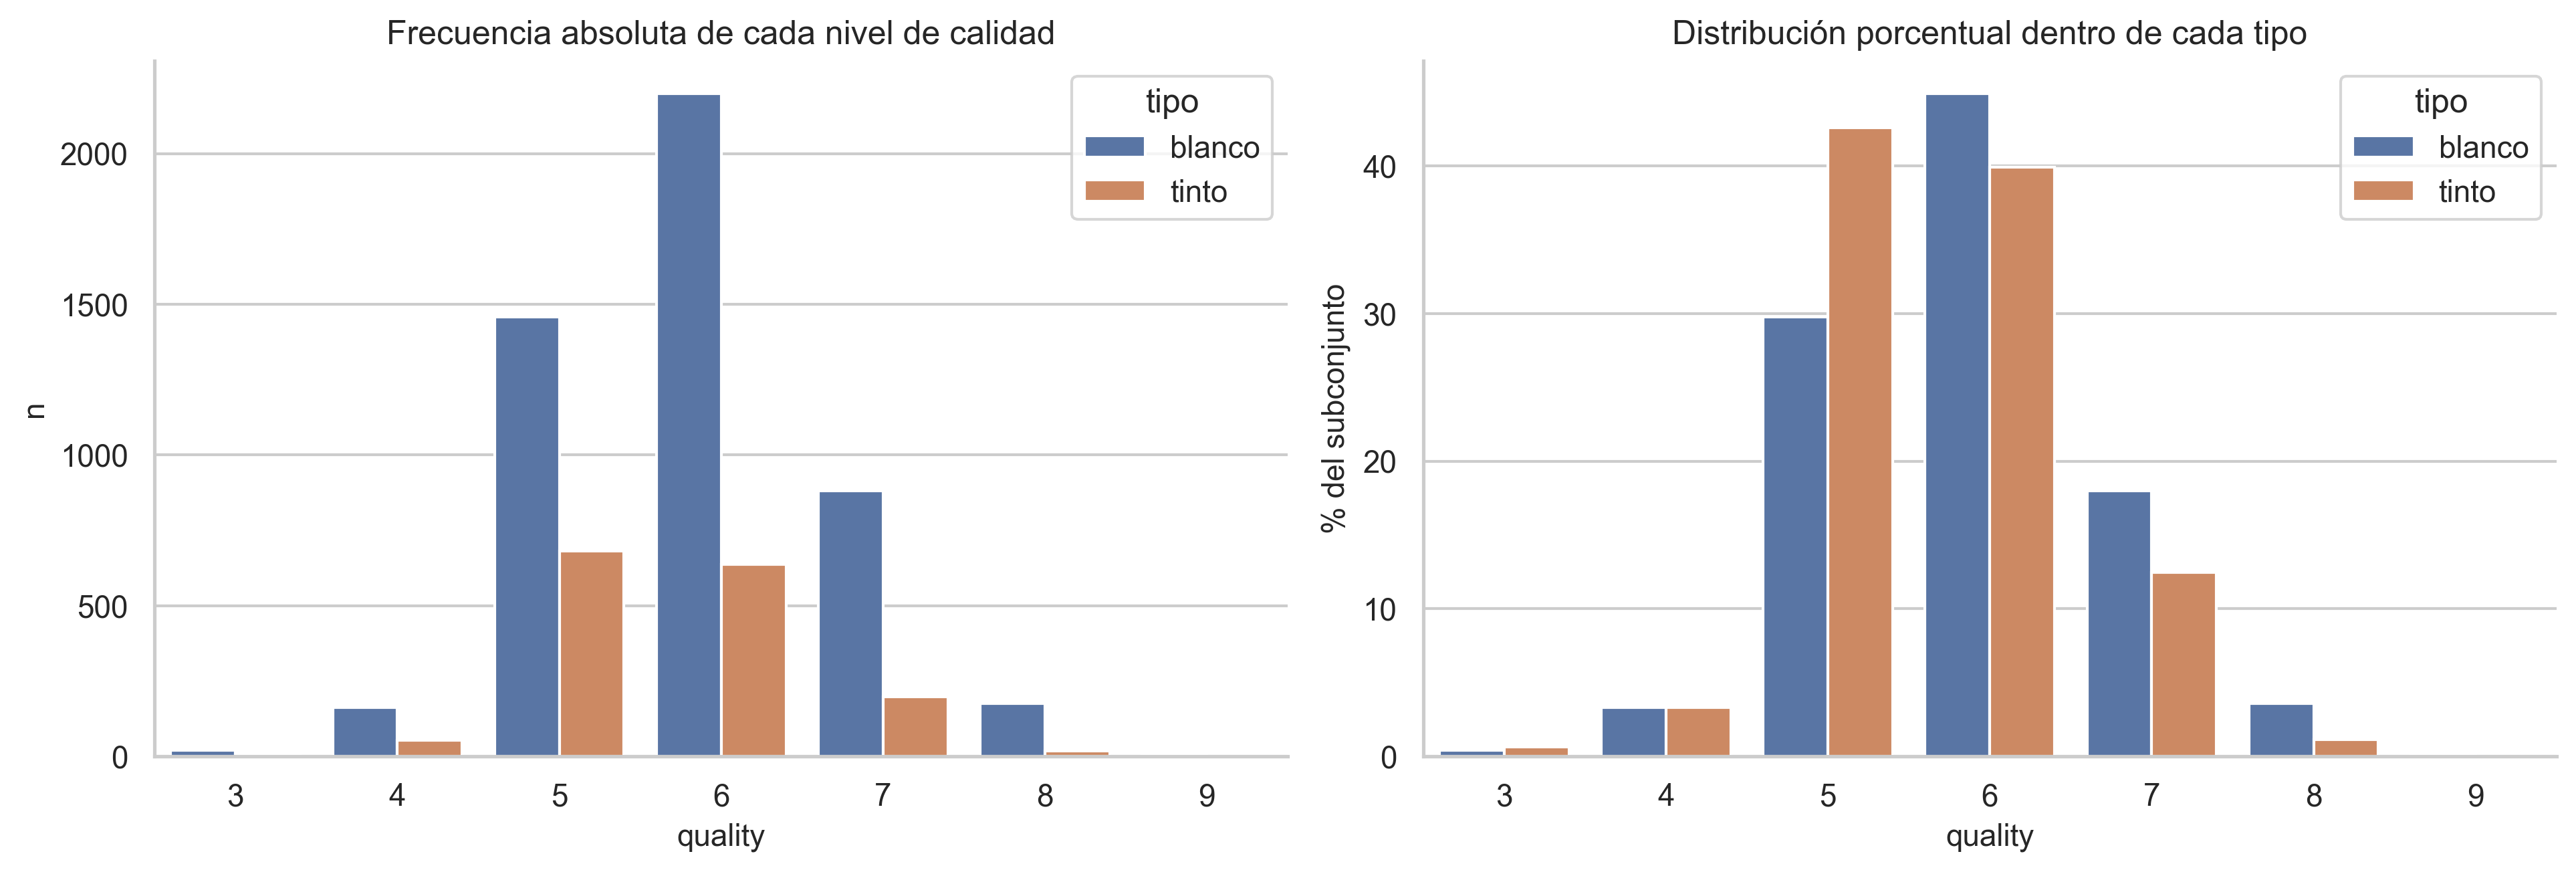
\includegraphics[width=\columnwidth]{fig_u2_03_quality_dist.png}
    \caption{Distribución de \texttt{quality} por tipo de vino.
             Las clases 5--7 concentran más del 90\,\% de las observaciones.}
    \label{fig:quality-dist}
\end{figure}

\subsection{Análisis univariado: distribuciones y estadísticas descriptivas}

La Figura~\ref{fig:distribuciones} presenta los histogramas de las once
variables fisicoquímicas. \texttt{residual sugar}, \texttt{chlorides} y
\texttt{sulphates} exhiben asimetría positiva marcada ($|\text{skew}| > 1$),
con colas derechas extensas características de distribuciones lognormales.
\texttt{density} y \texttt{pH} son aproximadamente simétricas ($|\text{skew}|
< 0{,}5$). Estas diferencias de forma motivaron el uso de Yeo--Johnson en la
etapa de preprocesamiento.

\begin{figure}[t]
    \centering
    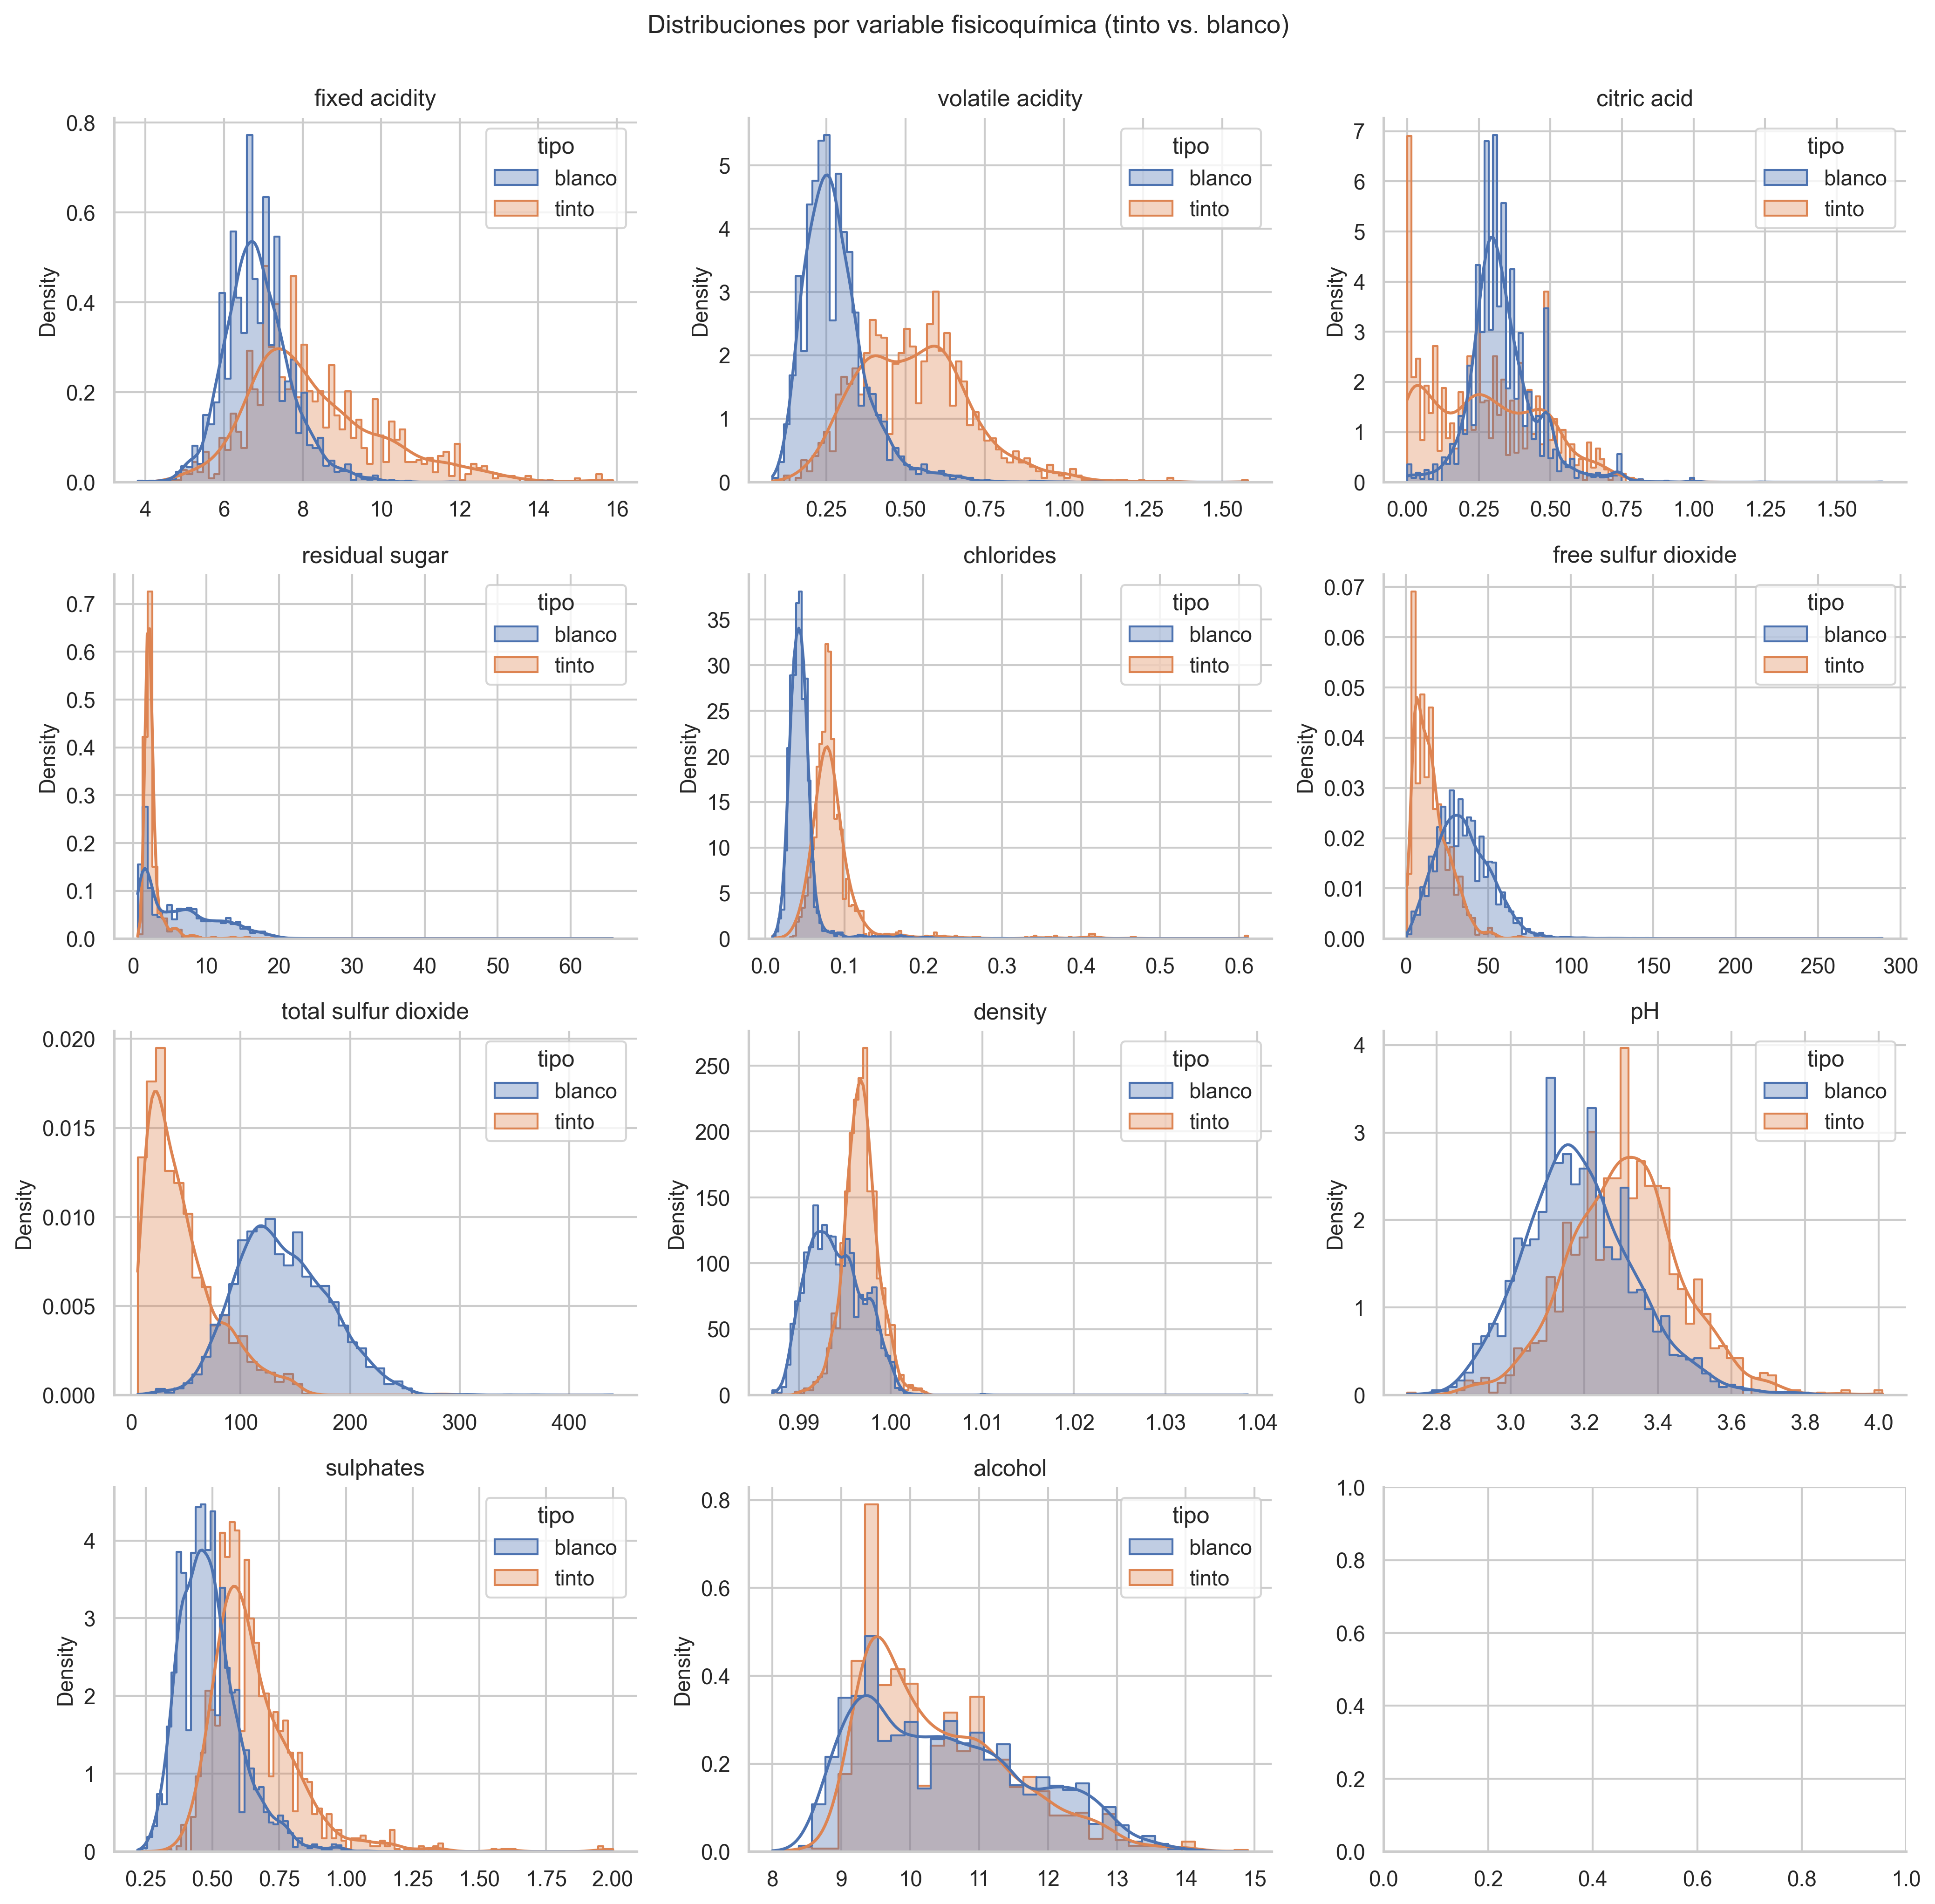
\includegraphics[width=\columnwidth]{fig_u2_01_distribuciones.png}
    \caption{Distribuciones de las once variables fisicoquímicas.
             Variables con cola derecha larga son candidatas a transformación.}
    \label{fig:distribuciones}
\end{figure}

\subsection{Relaciones entre variables y calidad}

La Figura~\ref{fig:correlaciones} muestra las matrices de correlación de
Pearson y Spearman. El ranking por $|\rho_{\text{Spearman}}|$ con
\texttt{quality} ubica a \texttt{alcohol} ($\rho \approx 0{,}45$) como la
variable de mayor asociación monótona, seguida de \texttt{density}
($\rho \approx -0{,}32$), \texttt{chlorides} ($\rho \approx -0{,}30$) y
\texttt{volatile acidity} ($\rho \approx -0{,}26$). Las diferencias entre
las matrices de Pearson y Spearman son moderadas, lo que sugiere relaciones
principalmente monótonas con algunas no linealidades locales.

\begin{figure}[t]
    \centering
    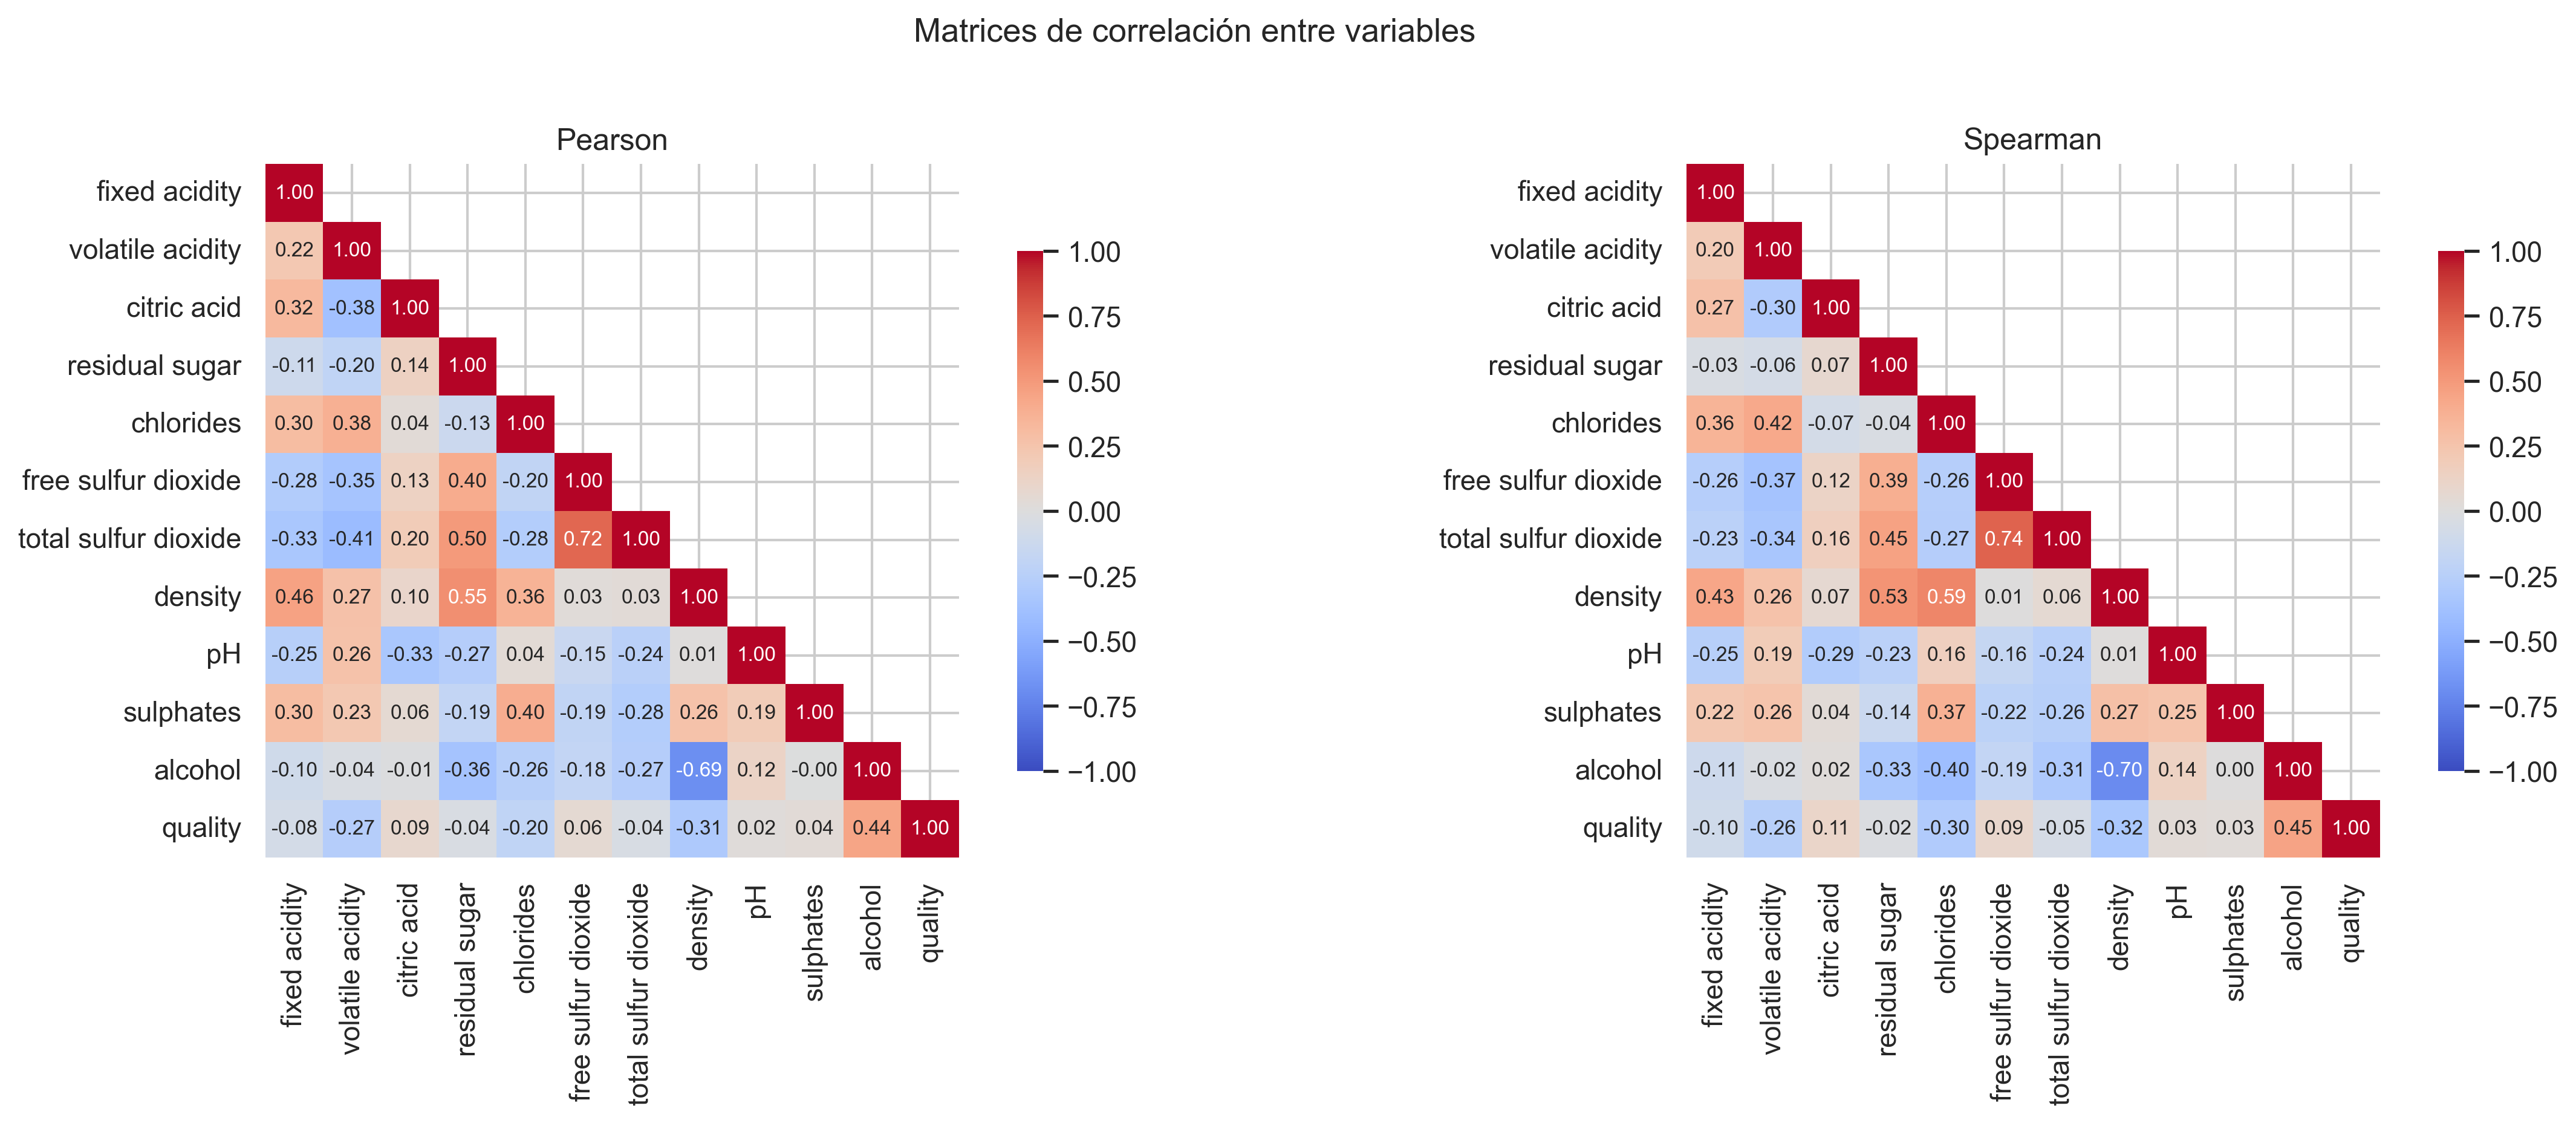
\includegraphics[width=\columnwidth]{fig_u2_04_correlaciones.png}
    \caption{Matrices de correlación de Pearson (izquierda) y Spearman
             (derecha) sobre el conjunto unificado.}
    \label{fig:correlaciones}
\end{figure}

La comparación por tipo (Fig.~\ref{fig:boxplots-tipo}) revela diferencias
estructurales marcadas en \texttt{total sulfur dioxide}, \texttt{volatile
acidity}, \texttt{free sulfur dioxide} y \texttt{chlorides}: los blancos
presentan mayor contenido de SO$_2$ total, mientras que los tintos exhiben
mayor acidez volátil y mayor contenido de cloruros.

\begin{figure}[t]
    \centering
    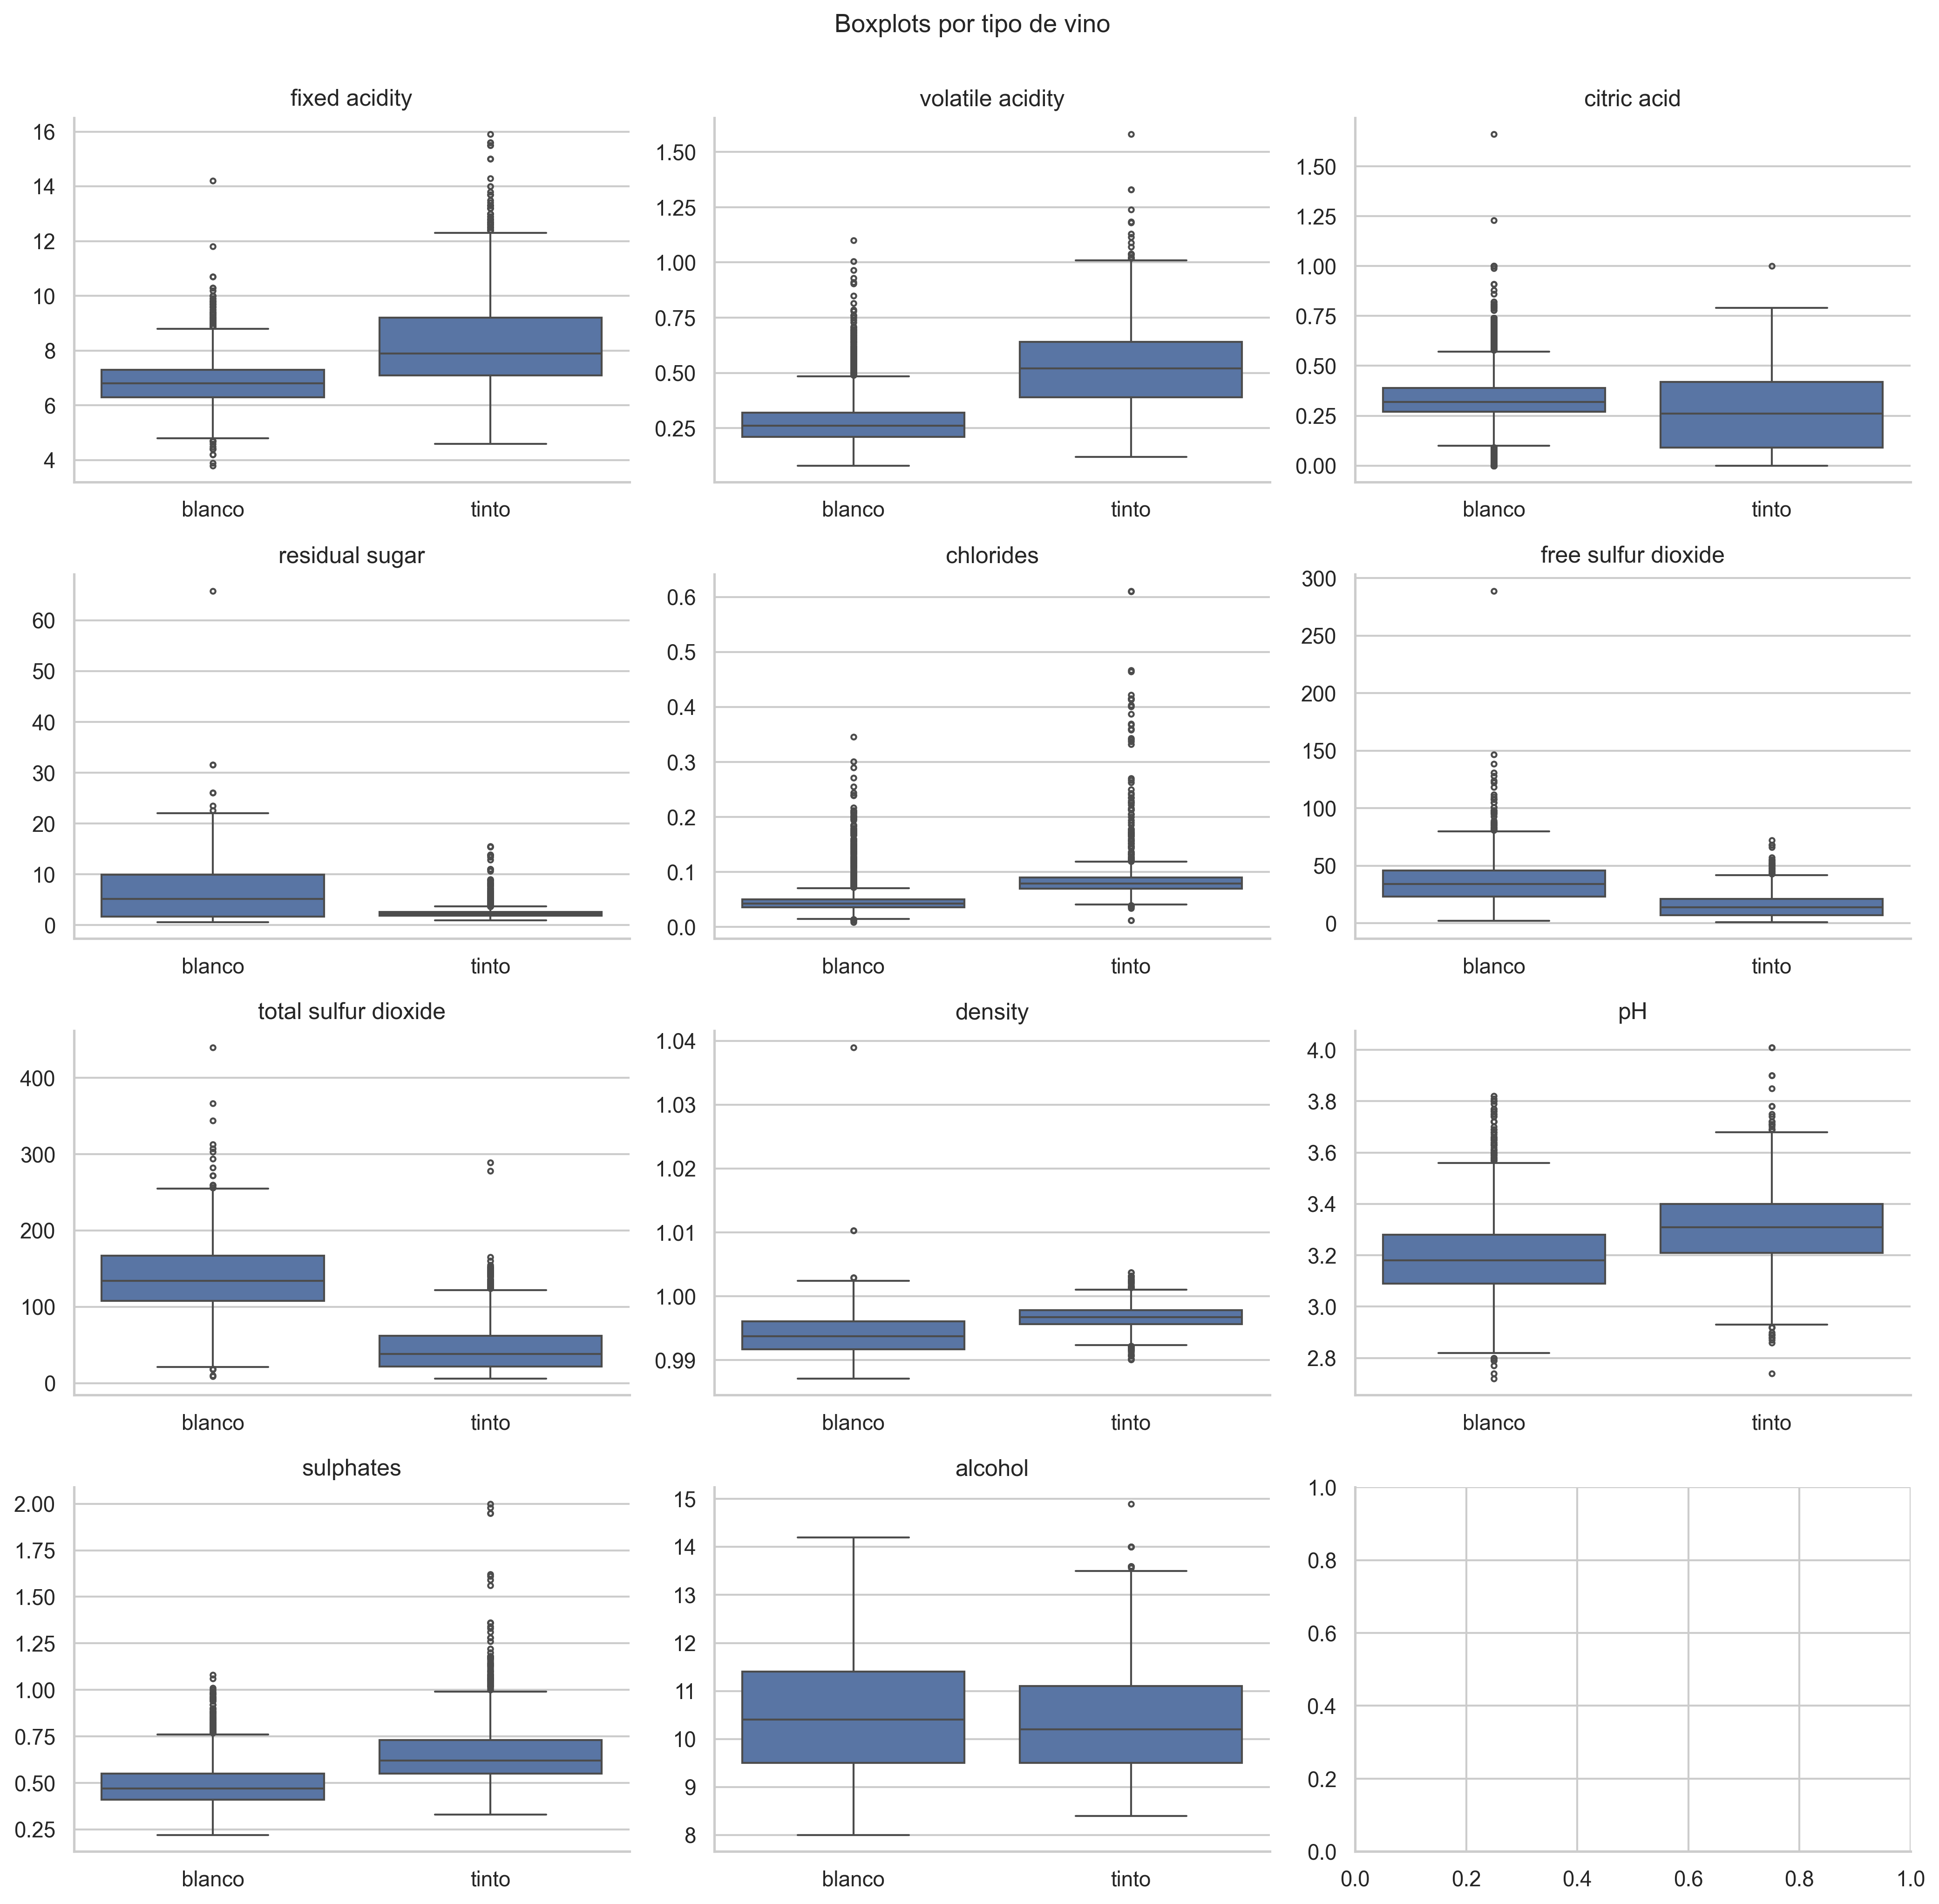
\includegraphics[width=\columnwidth]{fig_u2_02_boxplots_tipo.png}
    \caption{Diagramas de caja por tipo de vino para cada variable
             fisicoquímica. Se aprecia la separación estructural más marcada
             en \texttt{total\_sulfur\_dioxide} y \texttt{volatile\_acidity}.}
    \label{fig:boxplots-tipo}
\end{figure}

La prueba $\chi^2$ sobre \texttt{tipo} vs.\ \texttt{quality} discretizada
confirmó asociación estadísticamente significativa. Sin embargo, la V de
Cramér ($\approx 0{,}09$) indica un tamaño del efecto pequeño: el tipo de
vino influye en la calidad percibida pero no la determina.

\subsection{Análisis multivariado: PCA}

La Figura~\ref{fig:pca-varianza} presenta el diagrama de codo del PCA. PC1
explica el 27,5\,\% de la varianza y PC2 el 17,2\,\%; se requieren cinco
componentes para acumular el 80\,\%. El biplot (Fig.~\ref{fig:pca-biplot})
muestra que \texttt{total sulfur dioxide}, \texttt{residual sugar} y
\texttt{free sulfur dioxide} tienen cargas negativas altas en PC1, mientras
que \texttt{volatile acidity}, \texttt{chlorides} y \texttt{sulphates} apuntan
en la dirección opuesta, lo que produce una separación nítida entre vinos
tintos y blancos sobre el eje de PC1.

\begin{figure}[t]
    \centering
    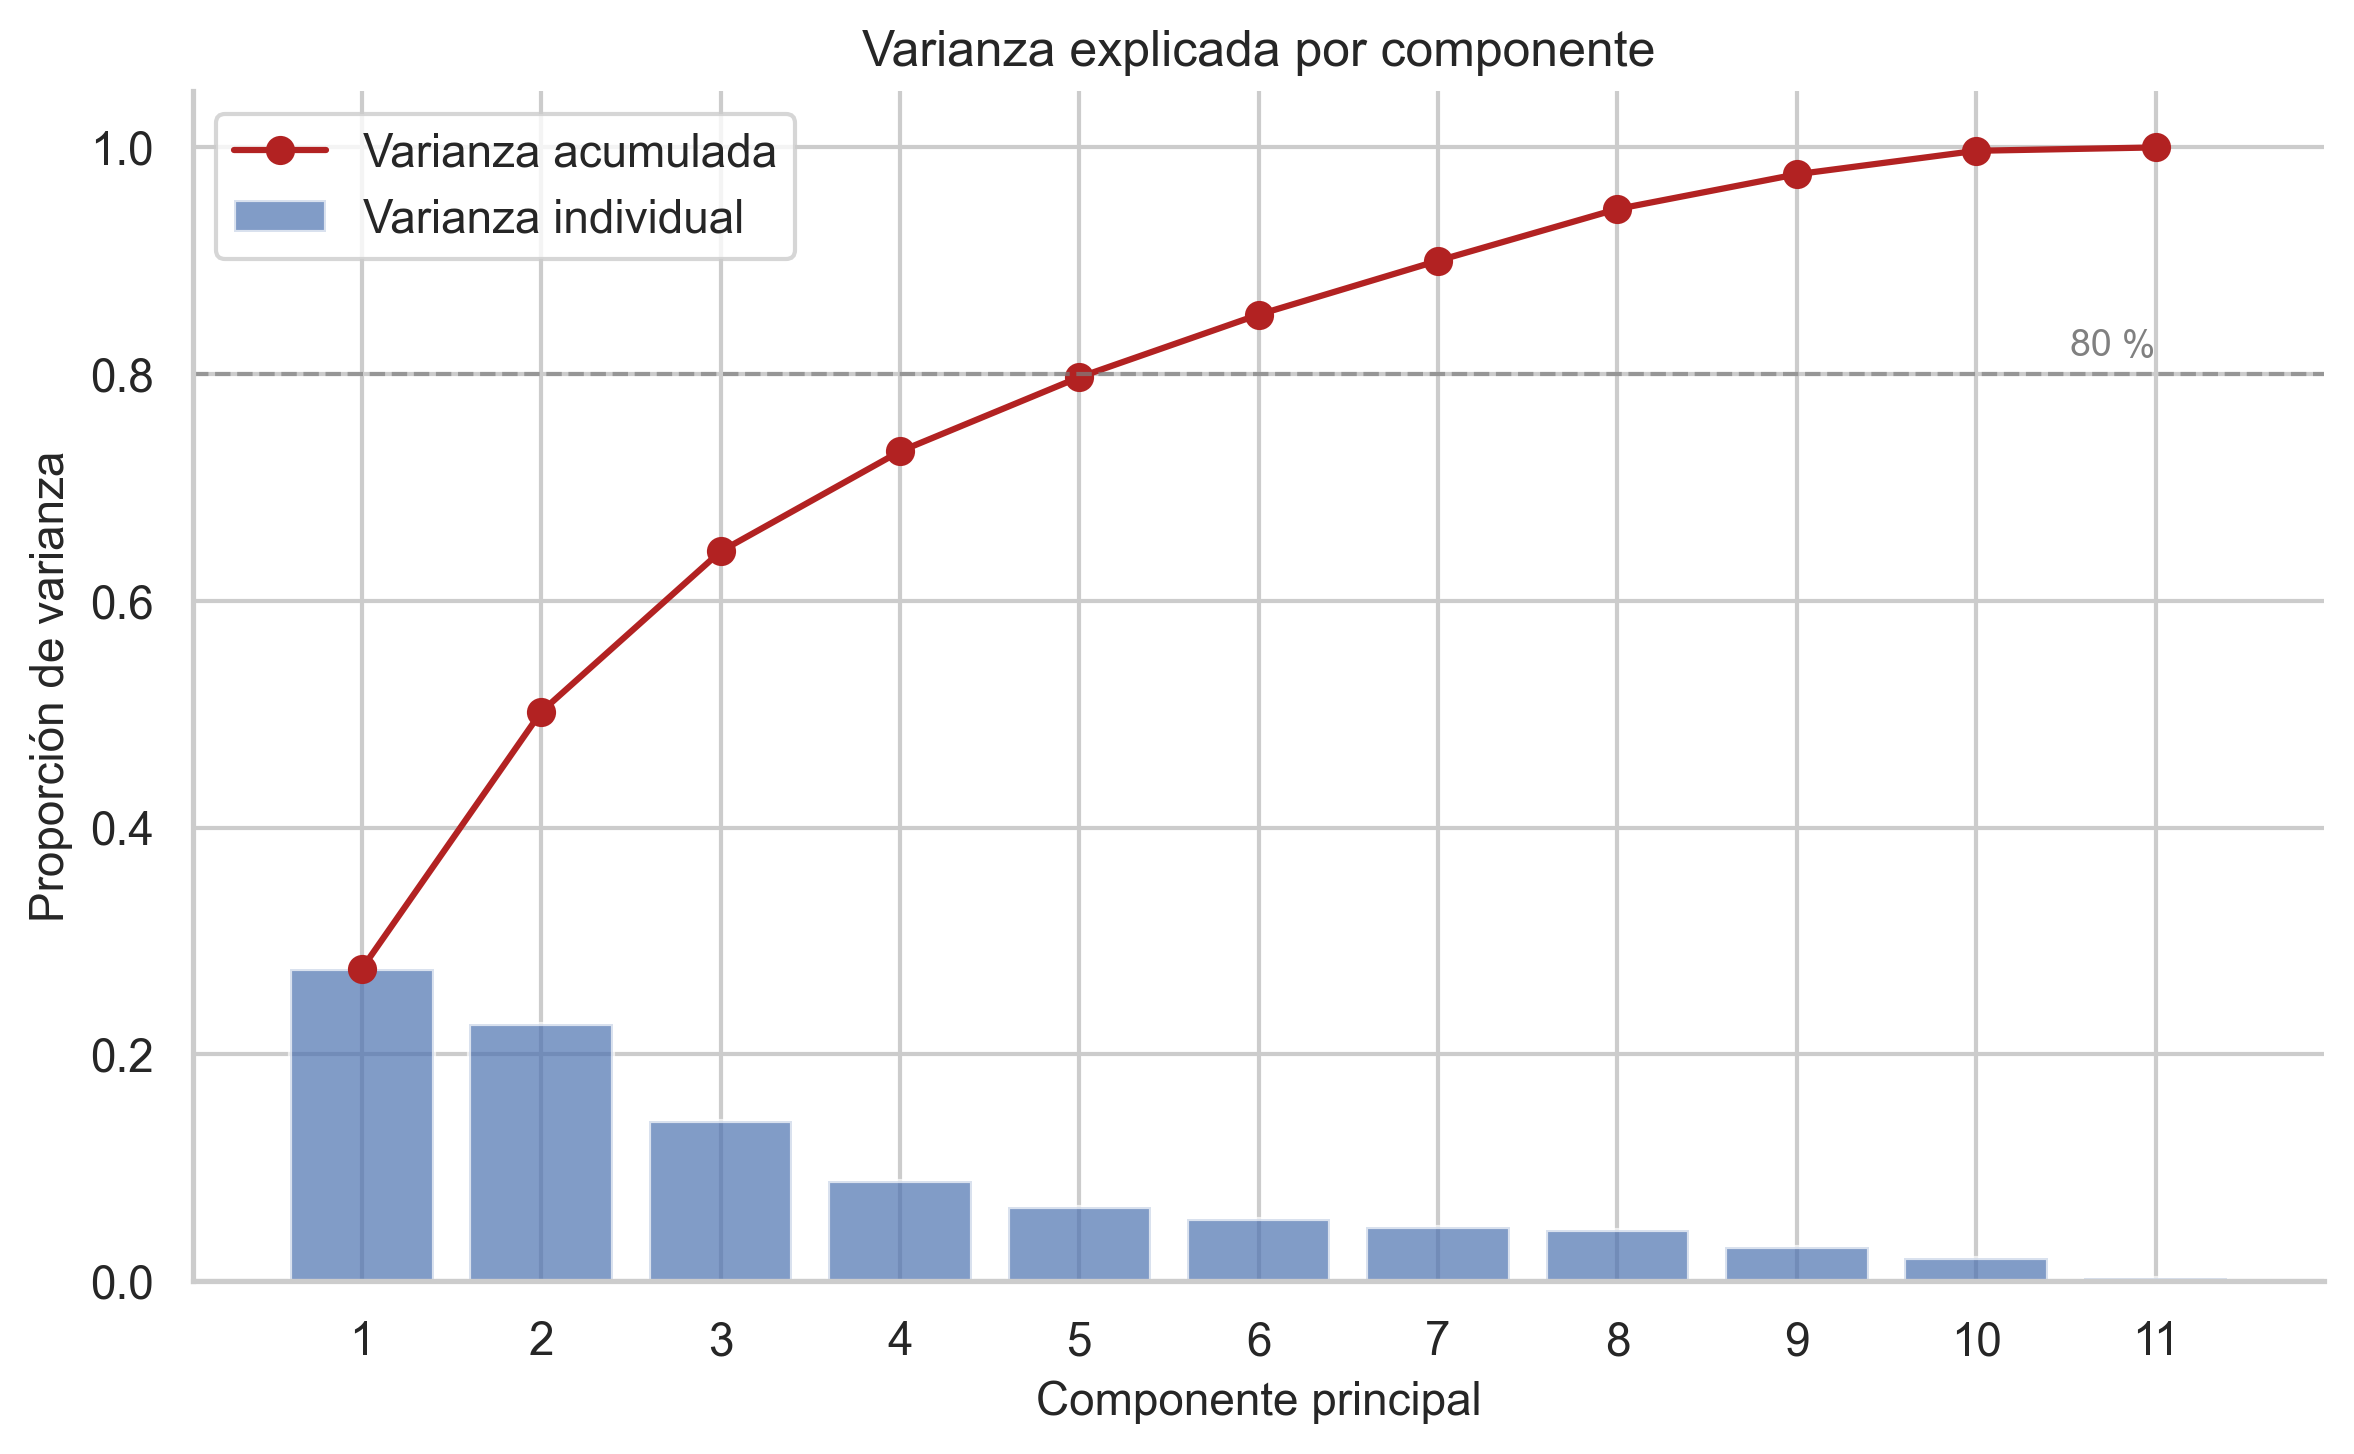
\includegraphics[width=\columnwidth]{fig_u2_06_pca_varianza.png}
    \caption{Diagrama de codo del PCA. PC1 explica el 27,5\,\% de la varianza;
             cinco componentes acumulan el 80\,\%.}
    \label{fig:pca-varianza}
\end{figure}

\begin{figure}[t]
    \centering
    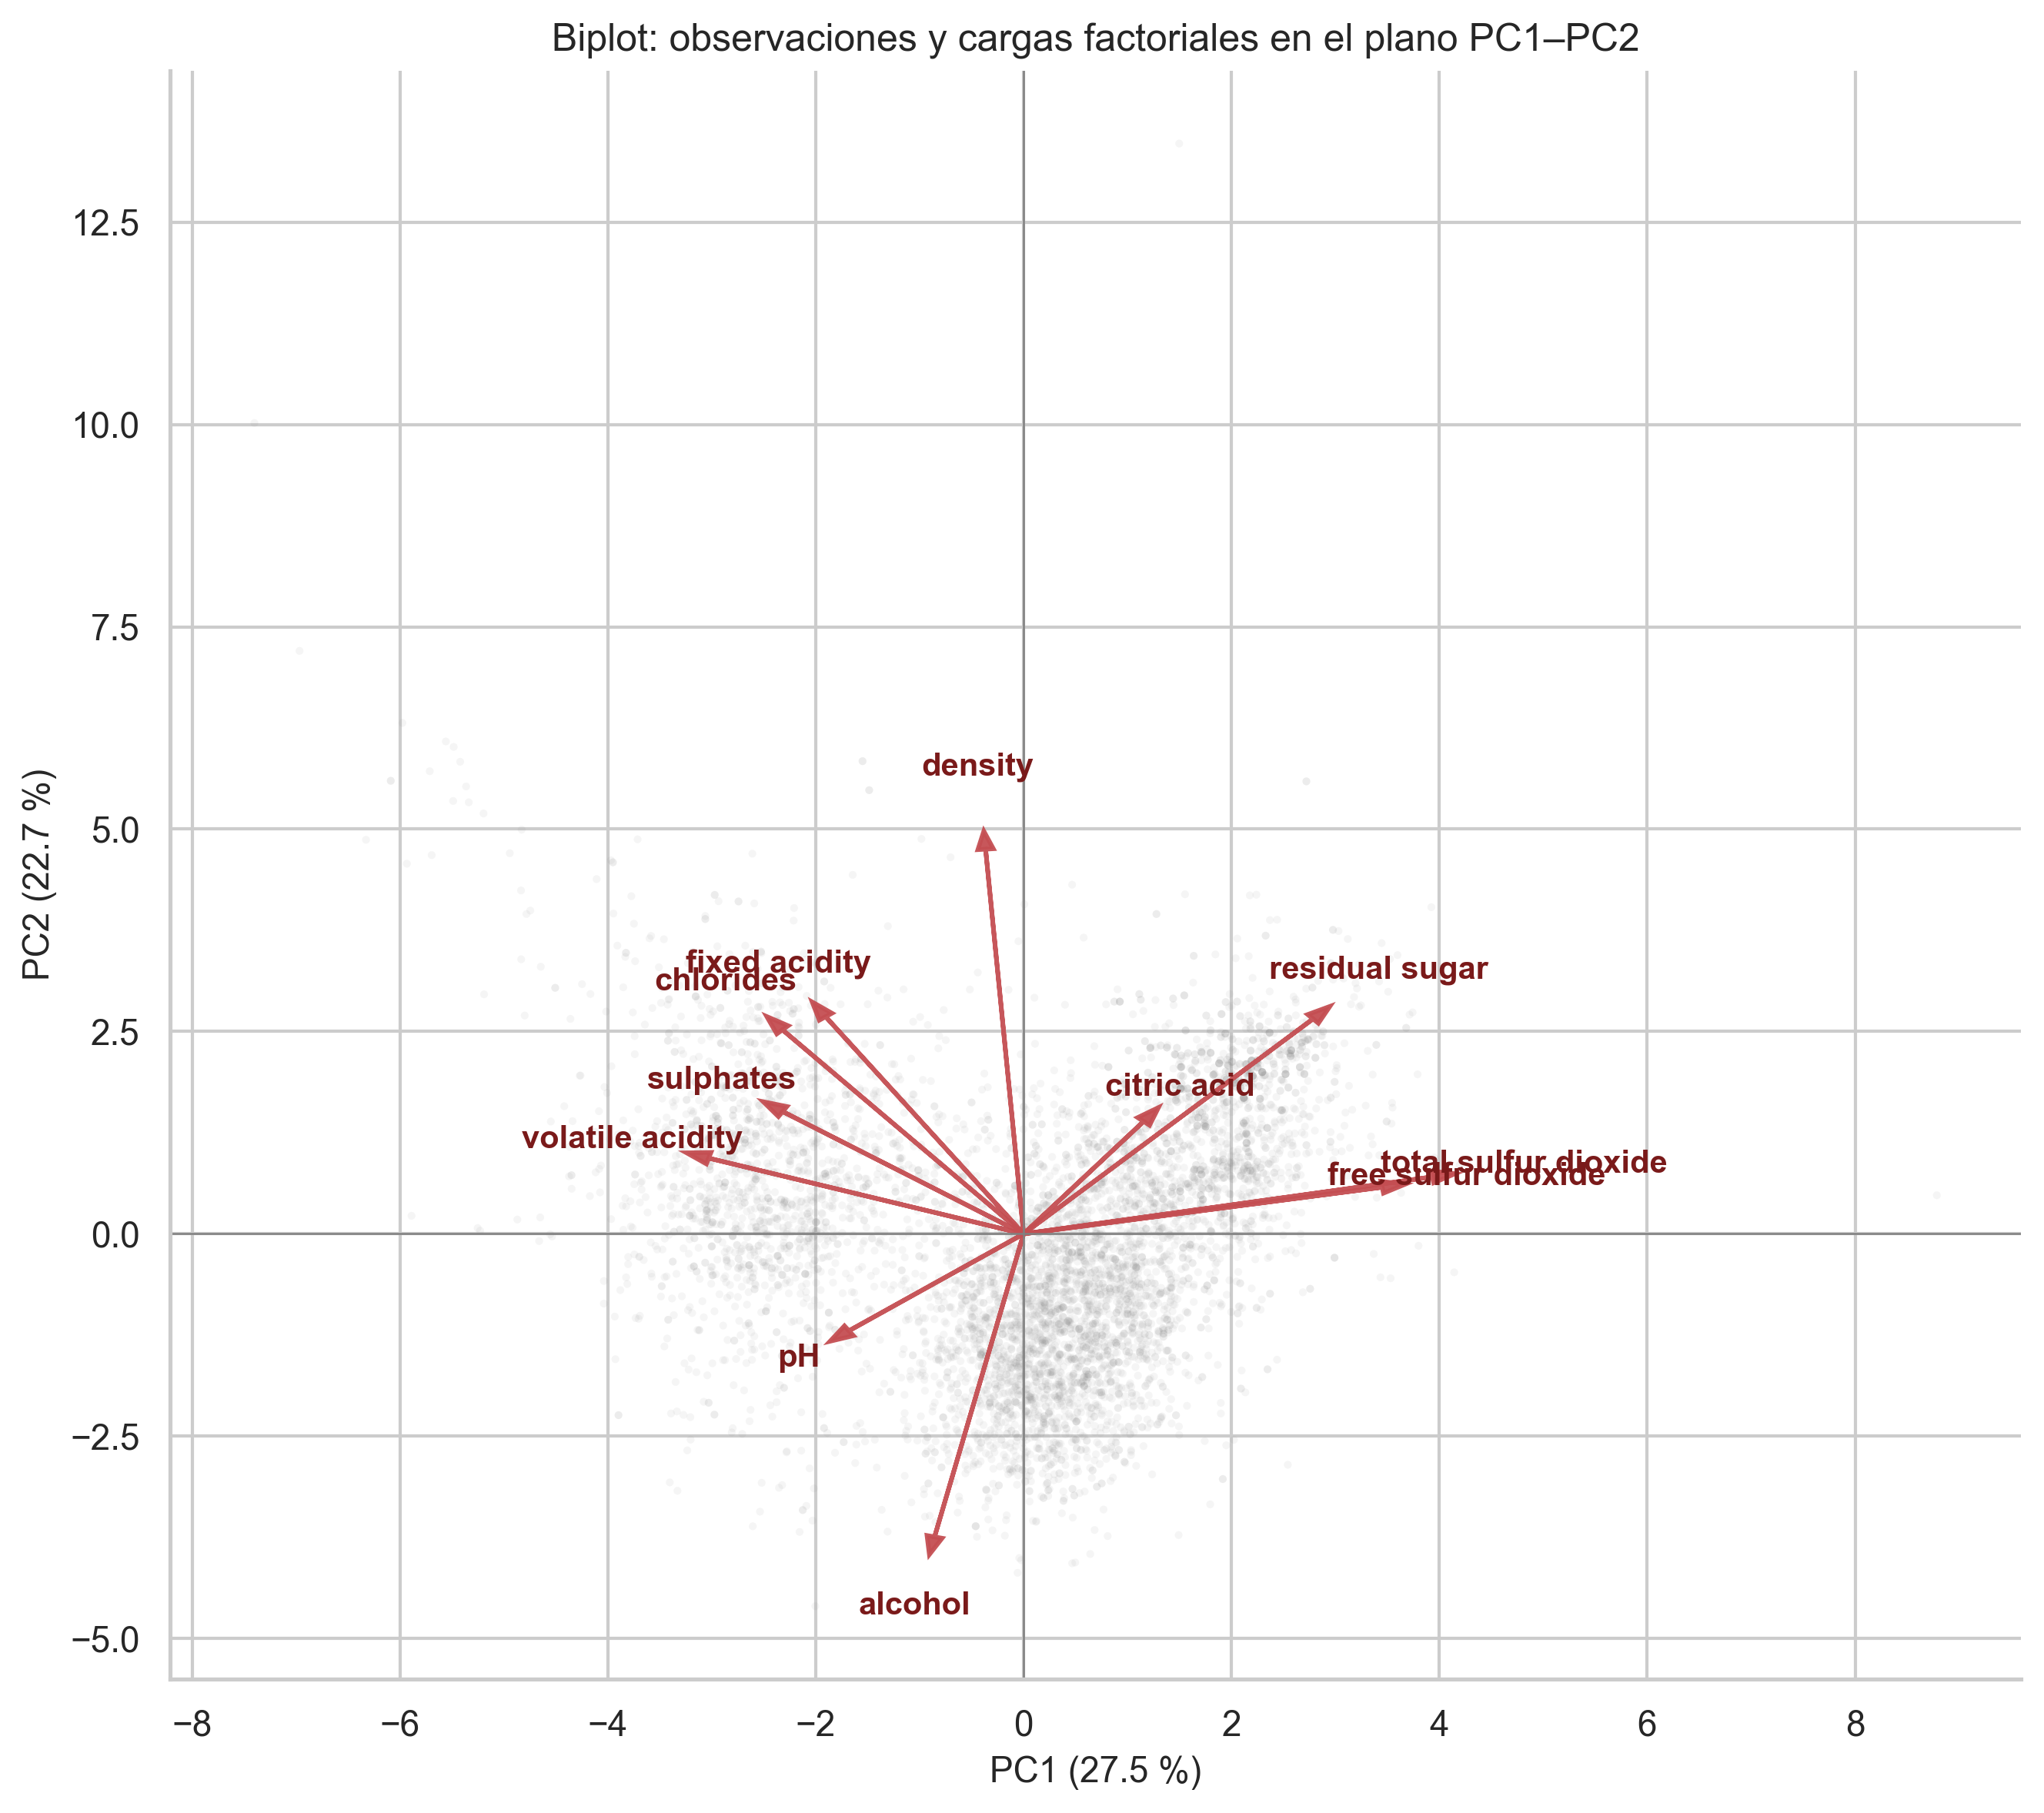
\includegraphics[width=\columnwidth]{fig_u2_08_pca_biplot.png}
    \caption{Biplot PCA (PC1--PC2). Los vectores de carga muestran
             las variables que mejor explican cada componente.
             PC1 discrimina tinto de blanco; PC2 captura
             el contraste densidad--alcohol.}
    \label{fig:pca-biplot}
\end{figure}

La proyección de las observaciones sobre el plano PC1--PC2 coloreada por
\texttt{quality} (Fig.~\ref{fig:pca-scatter}) presenta un gradiente difuso:
no existe una región del espacio reducido donde los vinos de alta o baja
calidad se concentren nítidamente. Este resultado anticipa que la predicción
de la calidad requerirá modelos capaces de capturar interacciones y no
linealidades.

\begin{figure}[t]
    \centering
    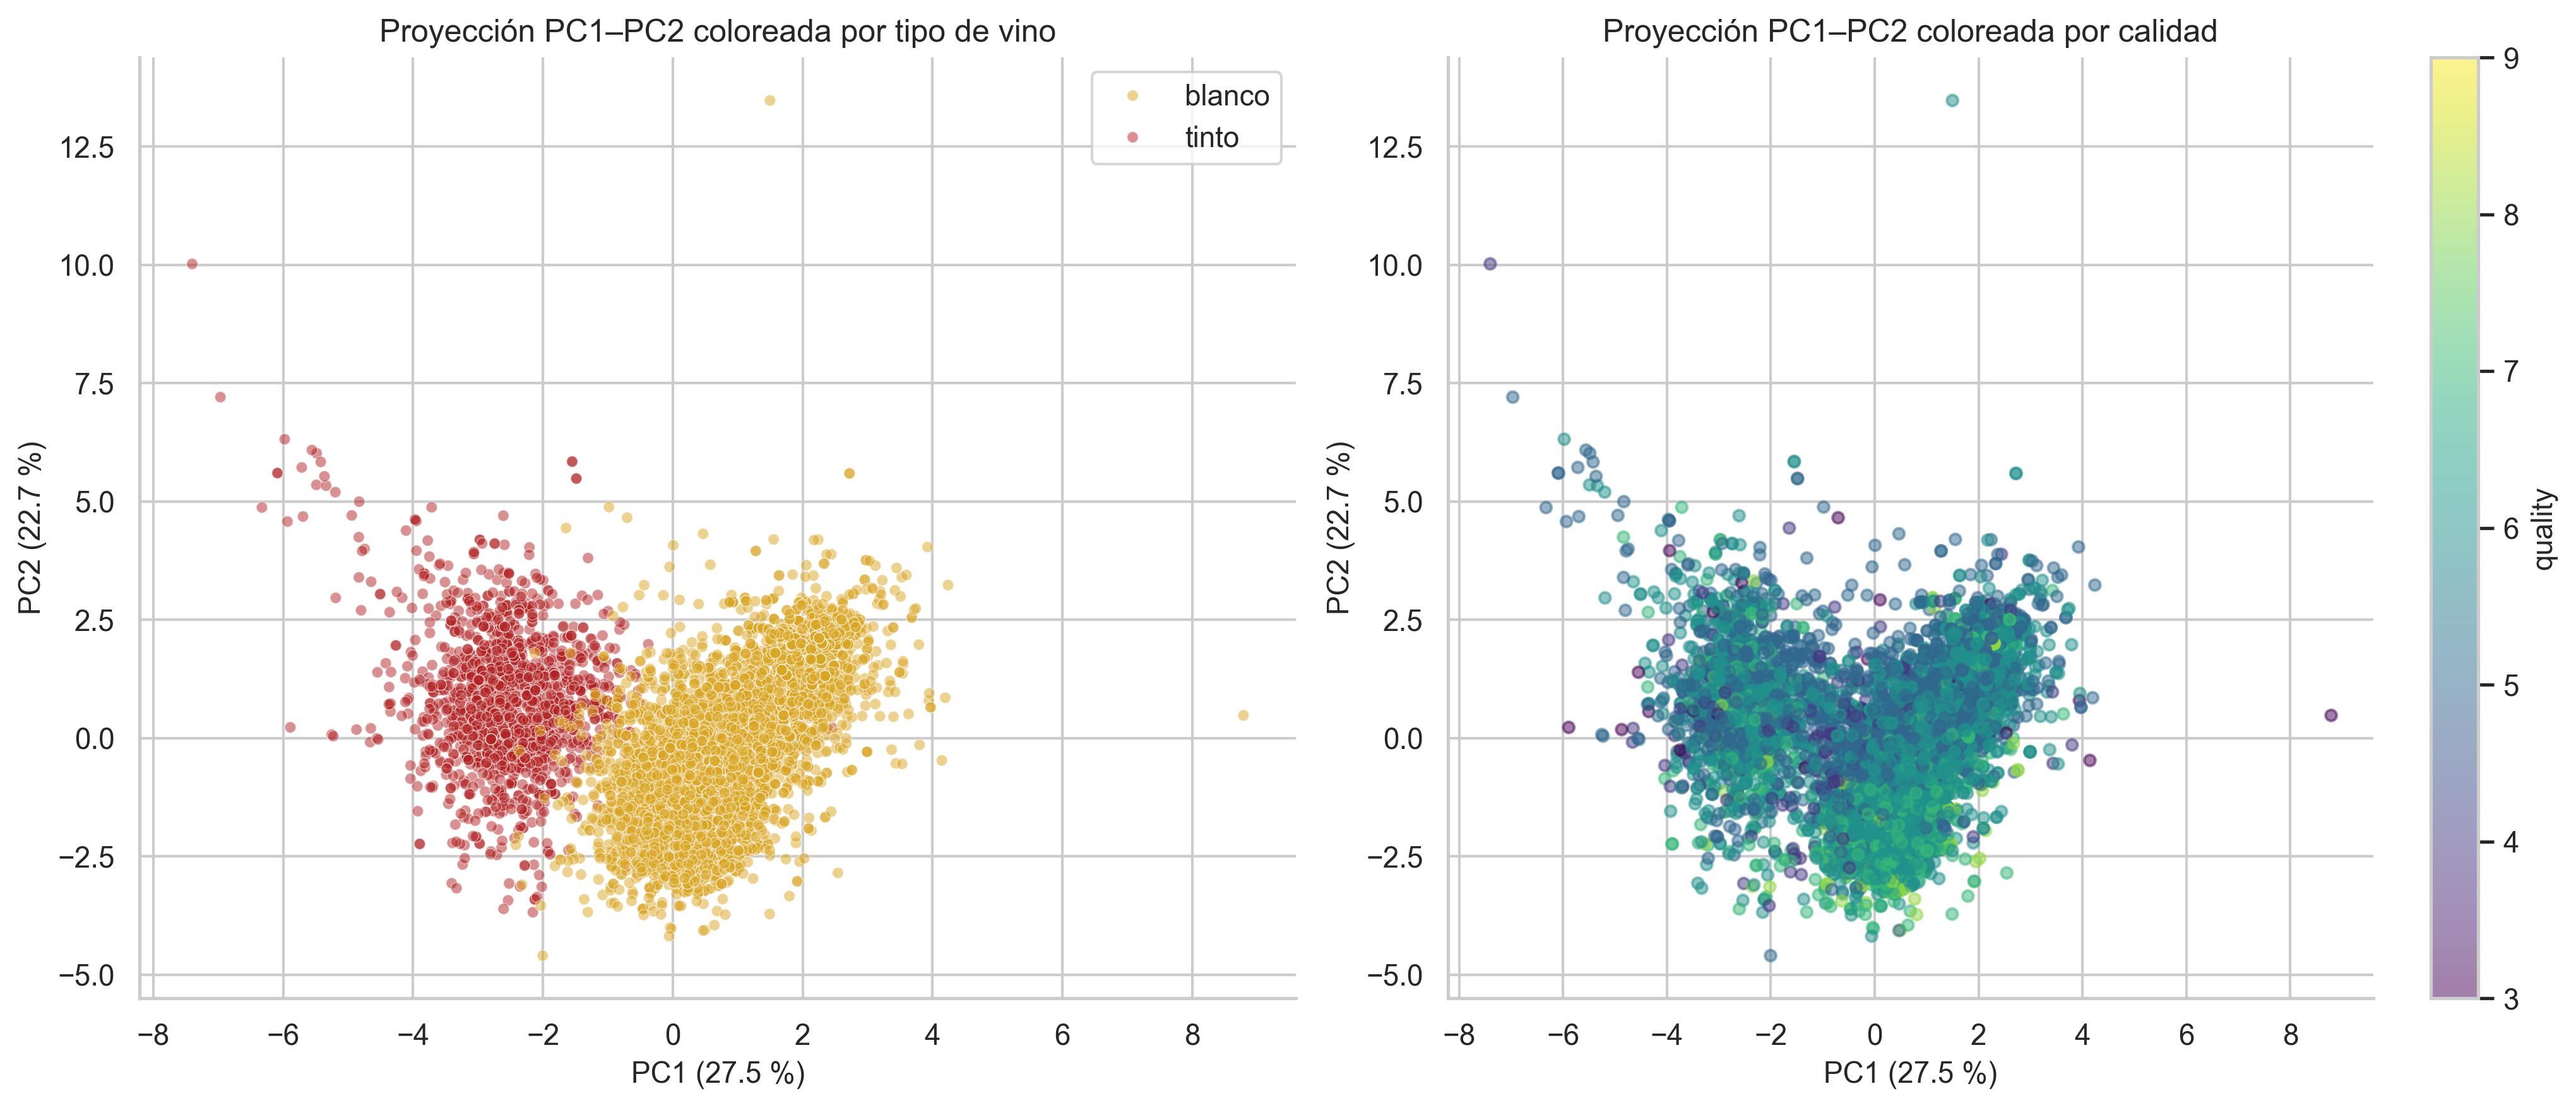
\includegraphics[width=\columnwidth]{fig_u2_07_pca_scatter.png}
    \caption{Proyección PCA coloreada por \texttt{quality}.
             El gradiente de calidad en el espacio PC1--PC2 es difuso,
             lo que indica que los componentes principales no
             discriminan directamente la calidad.}
    \label{fig:pca-scatter}
\end{figure}

\subsection{Detección de valores atípicos}

Los métodos estadísticos univariados detectaron la mayor cantidad de atípicos
en las variables con distribuciones sesgadas: \texttt{residual sugar},
\texttt{chlorides} y \texttt{sulphates}. La regla IQR resultó más sensible que
el puntaje~Z en este contexto, ya que la presencia de valores extremos infla
la desviación estándar muestral, ampliando el umbral $\pm 3s$ y reduciendo la
sensibilidad del criterio~Z.

Los métodos de aprendizaje automático (Isolation Forest y LOF), calibrados al
5\,\%, capturaron geometrías distintas de anomalía: Isolation Forest detecta
atípicos globales bien separados del conjunto, mientras que LOF identifica
puntos de baja densidad local (Fig.~\ref{fig:concordancia}). La coincidencia
exacta entre ambos métodos fue modesta, lo que refleja que cada algoritmo
opera sobre una noción diferente de anomalía. Las observaciones marcadas por
los cuatro métodos simultáneamente constituyeron menos del 2\,\% del conjunto
y representan los candidatos más sólidos a revisión manual.

\begin{figure}[t]
    \centering
    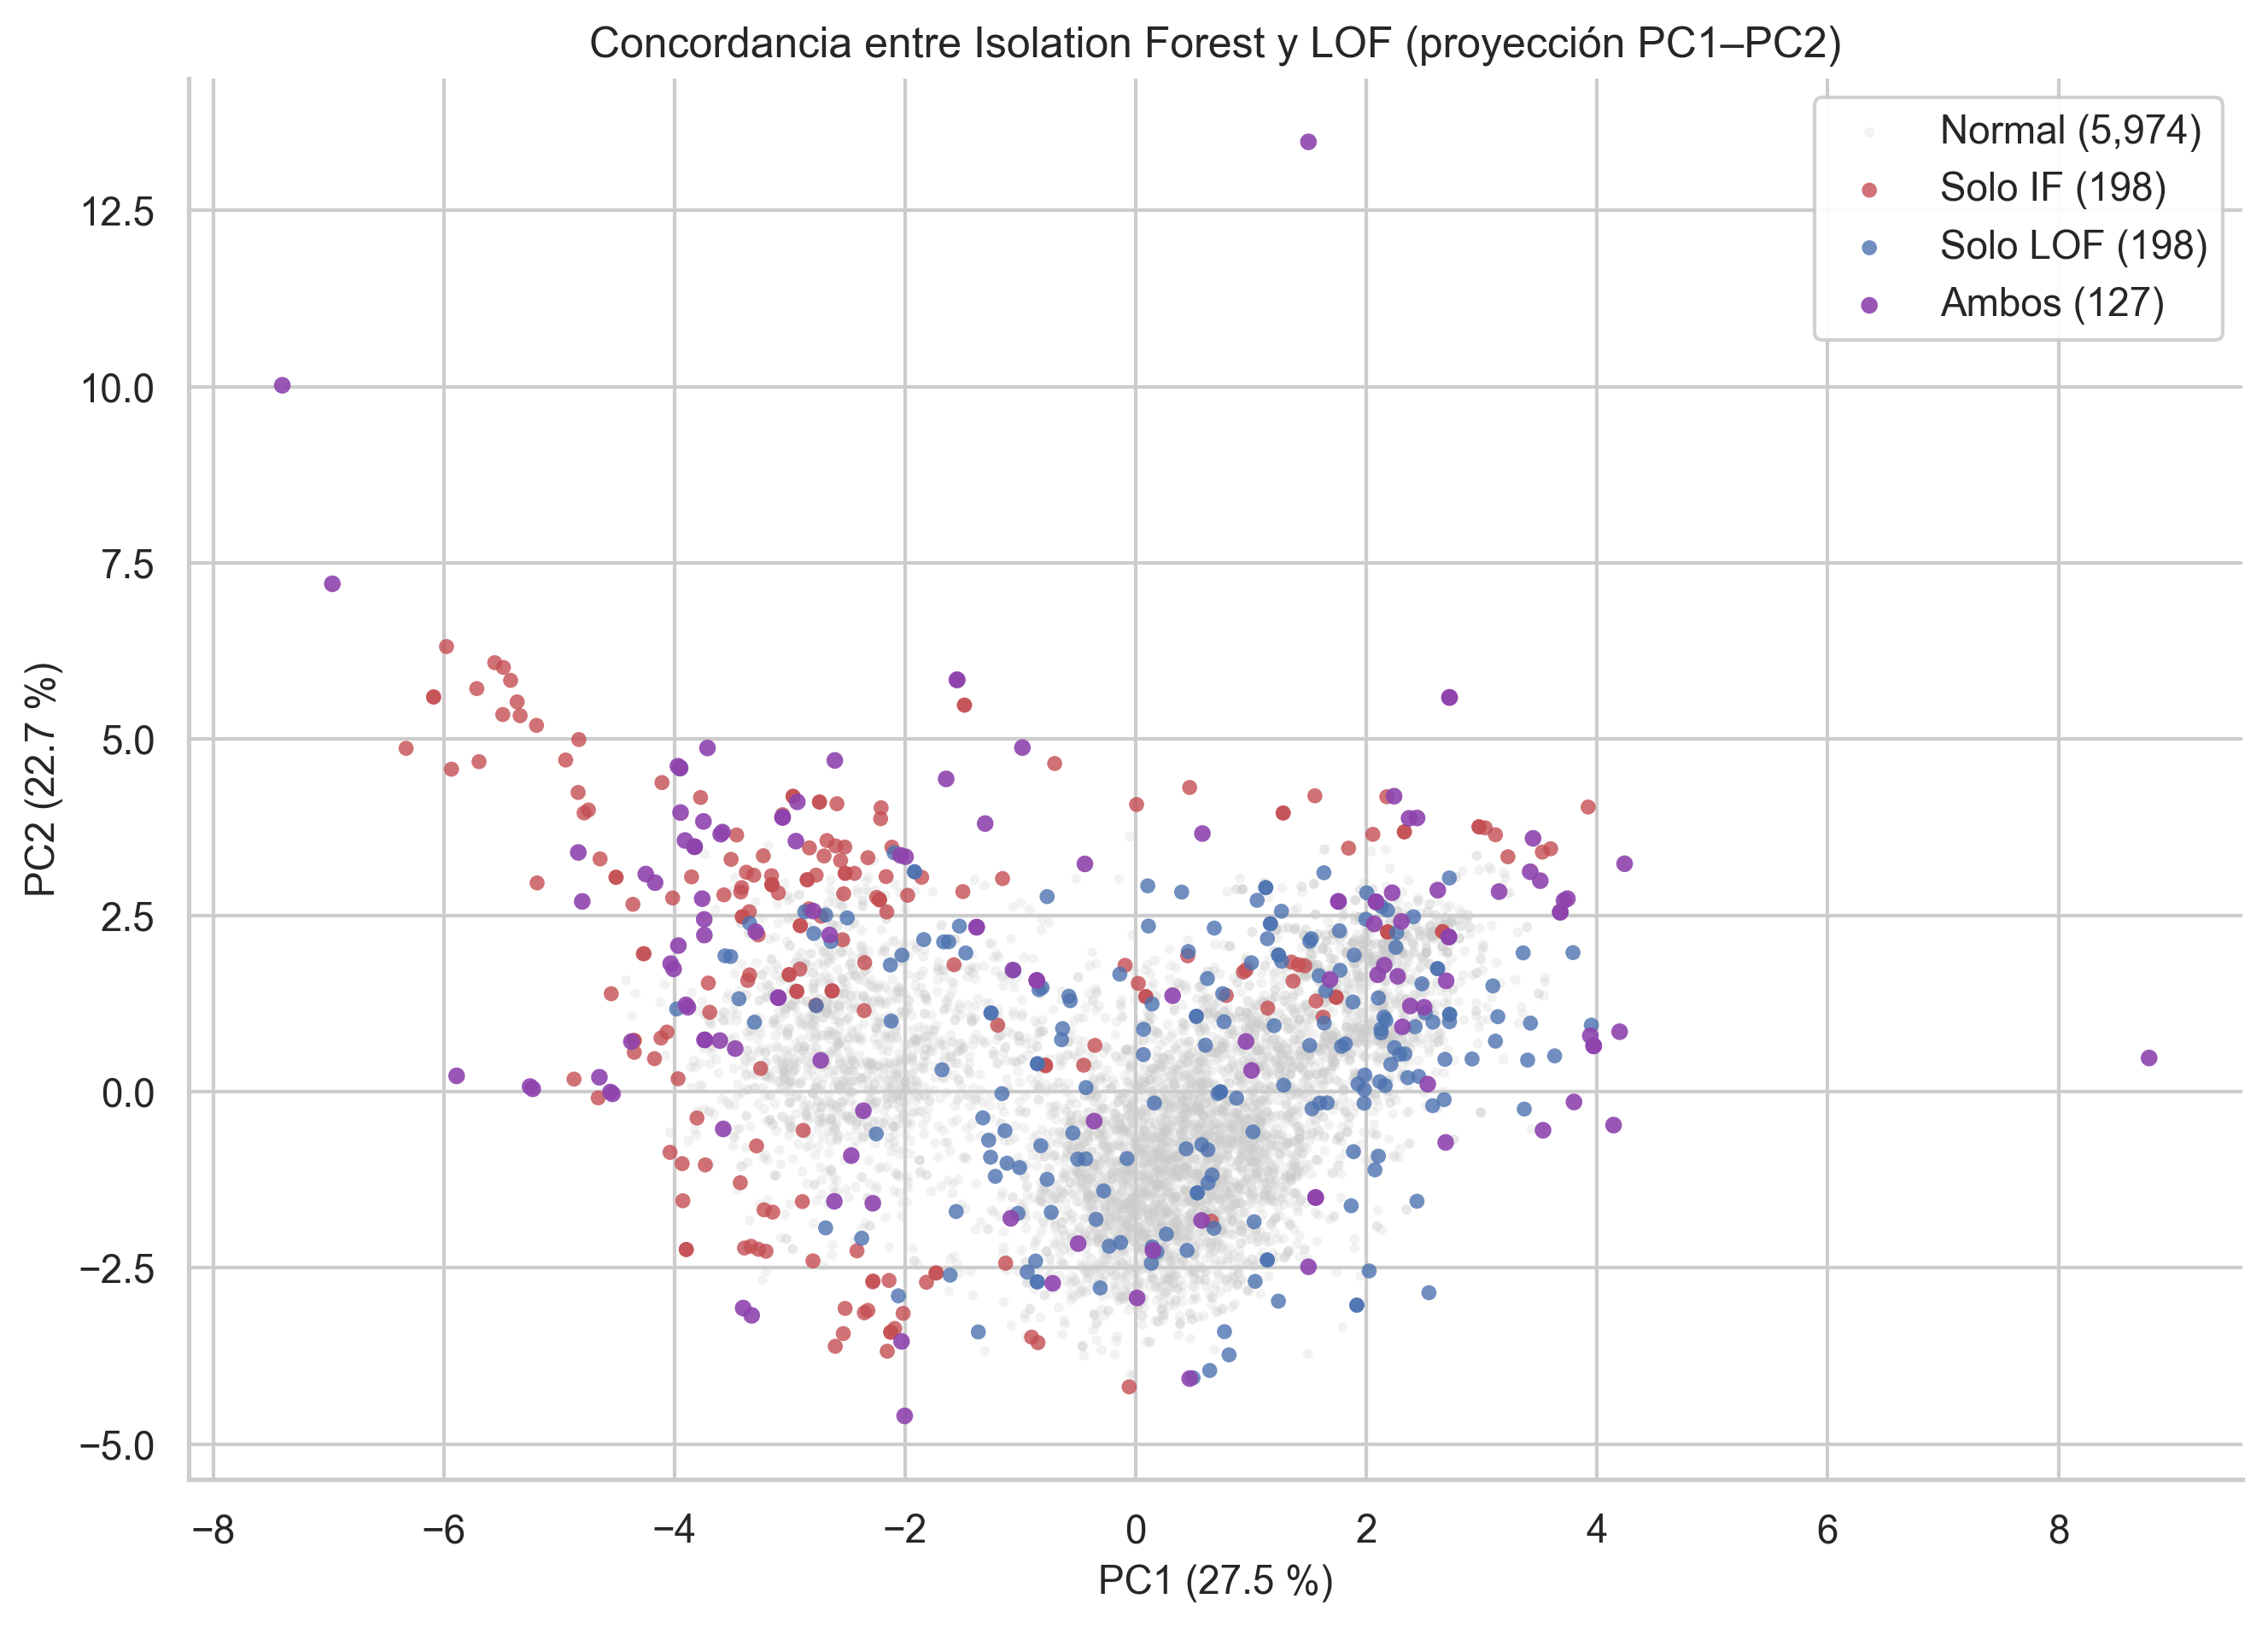
\includegraphics[width=\columnwidth]{fig_u3_03_concordancia_ml.png}
    \caption{Concordancia entre Isolation Forest y LOF.
             La superposición parcial refleja las distintas nociones de
             anomalía de cada método.}
    \label{fig:concordancia}
\end{figure}

Dado que las distribuciones son intrínsecamente asimétricas y los valores
extremos son químicamente plausibles, se optó por \textbf{no eliminar} los
atípicos univariados de forma indiscriminada, sino por tratarlos mediante
transformación Yeo--Johnson en la etapa de preprocesamiento.

\subsection{Preprocesamiento aplicado}

La Tabla~\ref{tab:pipeline} resume el flujo de preprocesamiento.

\begin{table}[t]
    \caption{Flujo de preprocesamiento del conjunto \textit{Wine Quality}}
    \label{tab:pipeline}
    \centering
    \begin{tabular}{lcc}
        \toprule
        \textbf{Etapa} & \textbf{Filas} & \textbf{Acción principal} \\
        \midrule
        Conjunto crudo unificado      & 6\,497 & --- \\
        Eliminación de duplicados     & 5\,320 & $-1\,177$ filas (18,1\,\%) \\
        Transformación Yeo--Johnson   & 5\,320 & Variables con $|\text{skew}|>1$ \\
        Escalamiento StandardScaler   & 5\,320 & Todas las fisicoquímicas \\
        Conjunto exportado            & 5\,320 & \texttt{winequality\_procesado.csv} \\
        \bottomrule
    \end{tabular}
\end{table}

Se eliminaron 1\,177 filas duplicadas exactas (18,1\,\% del conjunto crudo),
lo que reduce el conjunto a 5\,320 observaciones. Con fines demostrativos, se
simuló un escenario de valores faltantes completamente aleatorios (MCAR) al
5\,\% y se aplicó \texttt{KNNImputer} ($k = 5$) para su recuperación; la
Figura~\ref{fig:imputacion-knn} muestra que los valores imputados reproducen
la distribución original con error bajo, validando la estrategia.

\begin{figure}[t]
    \centering
    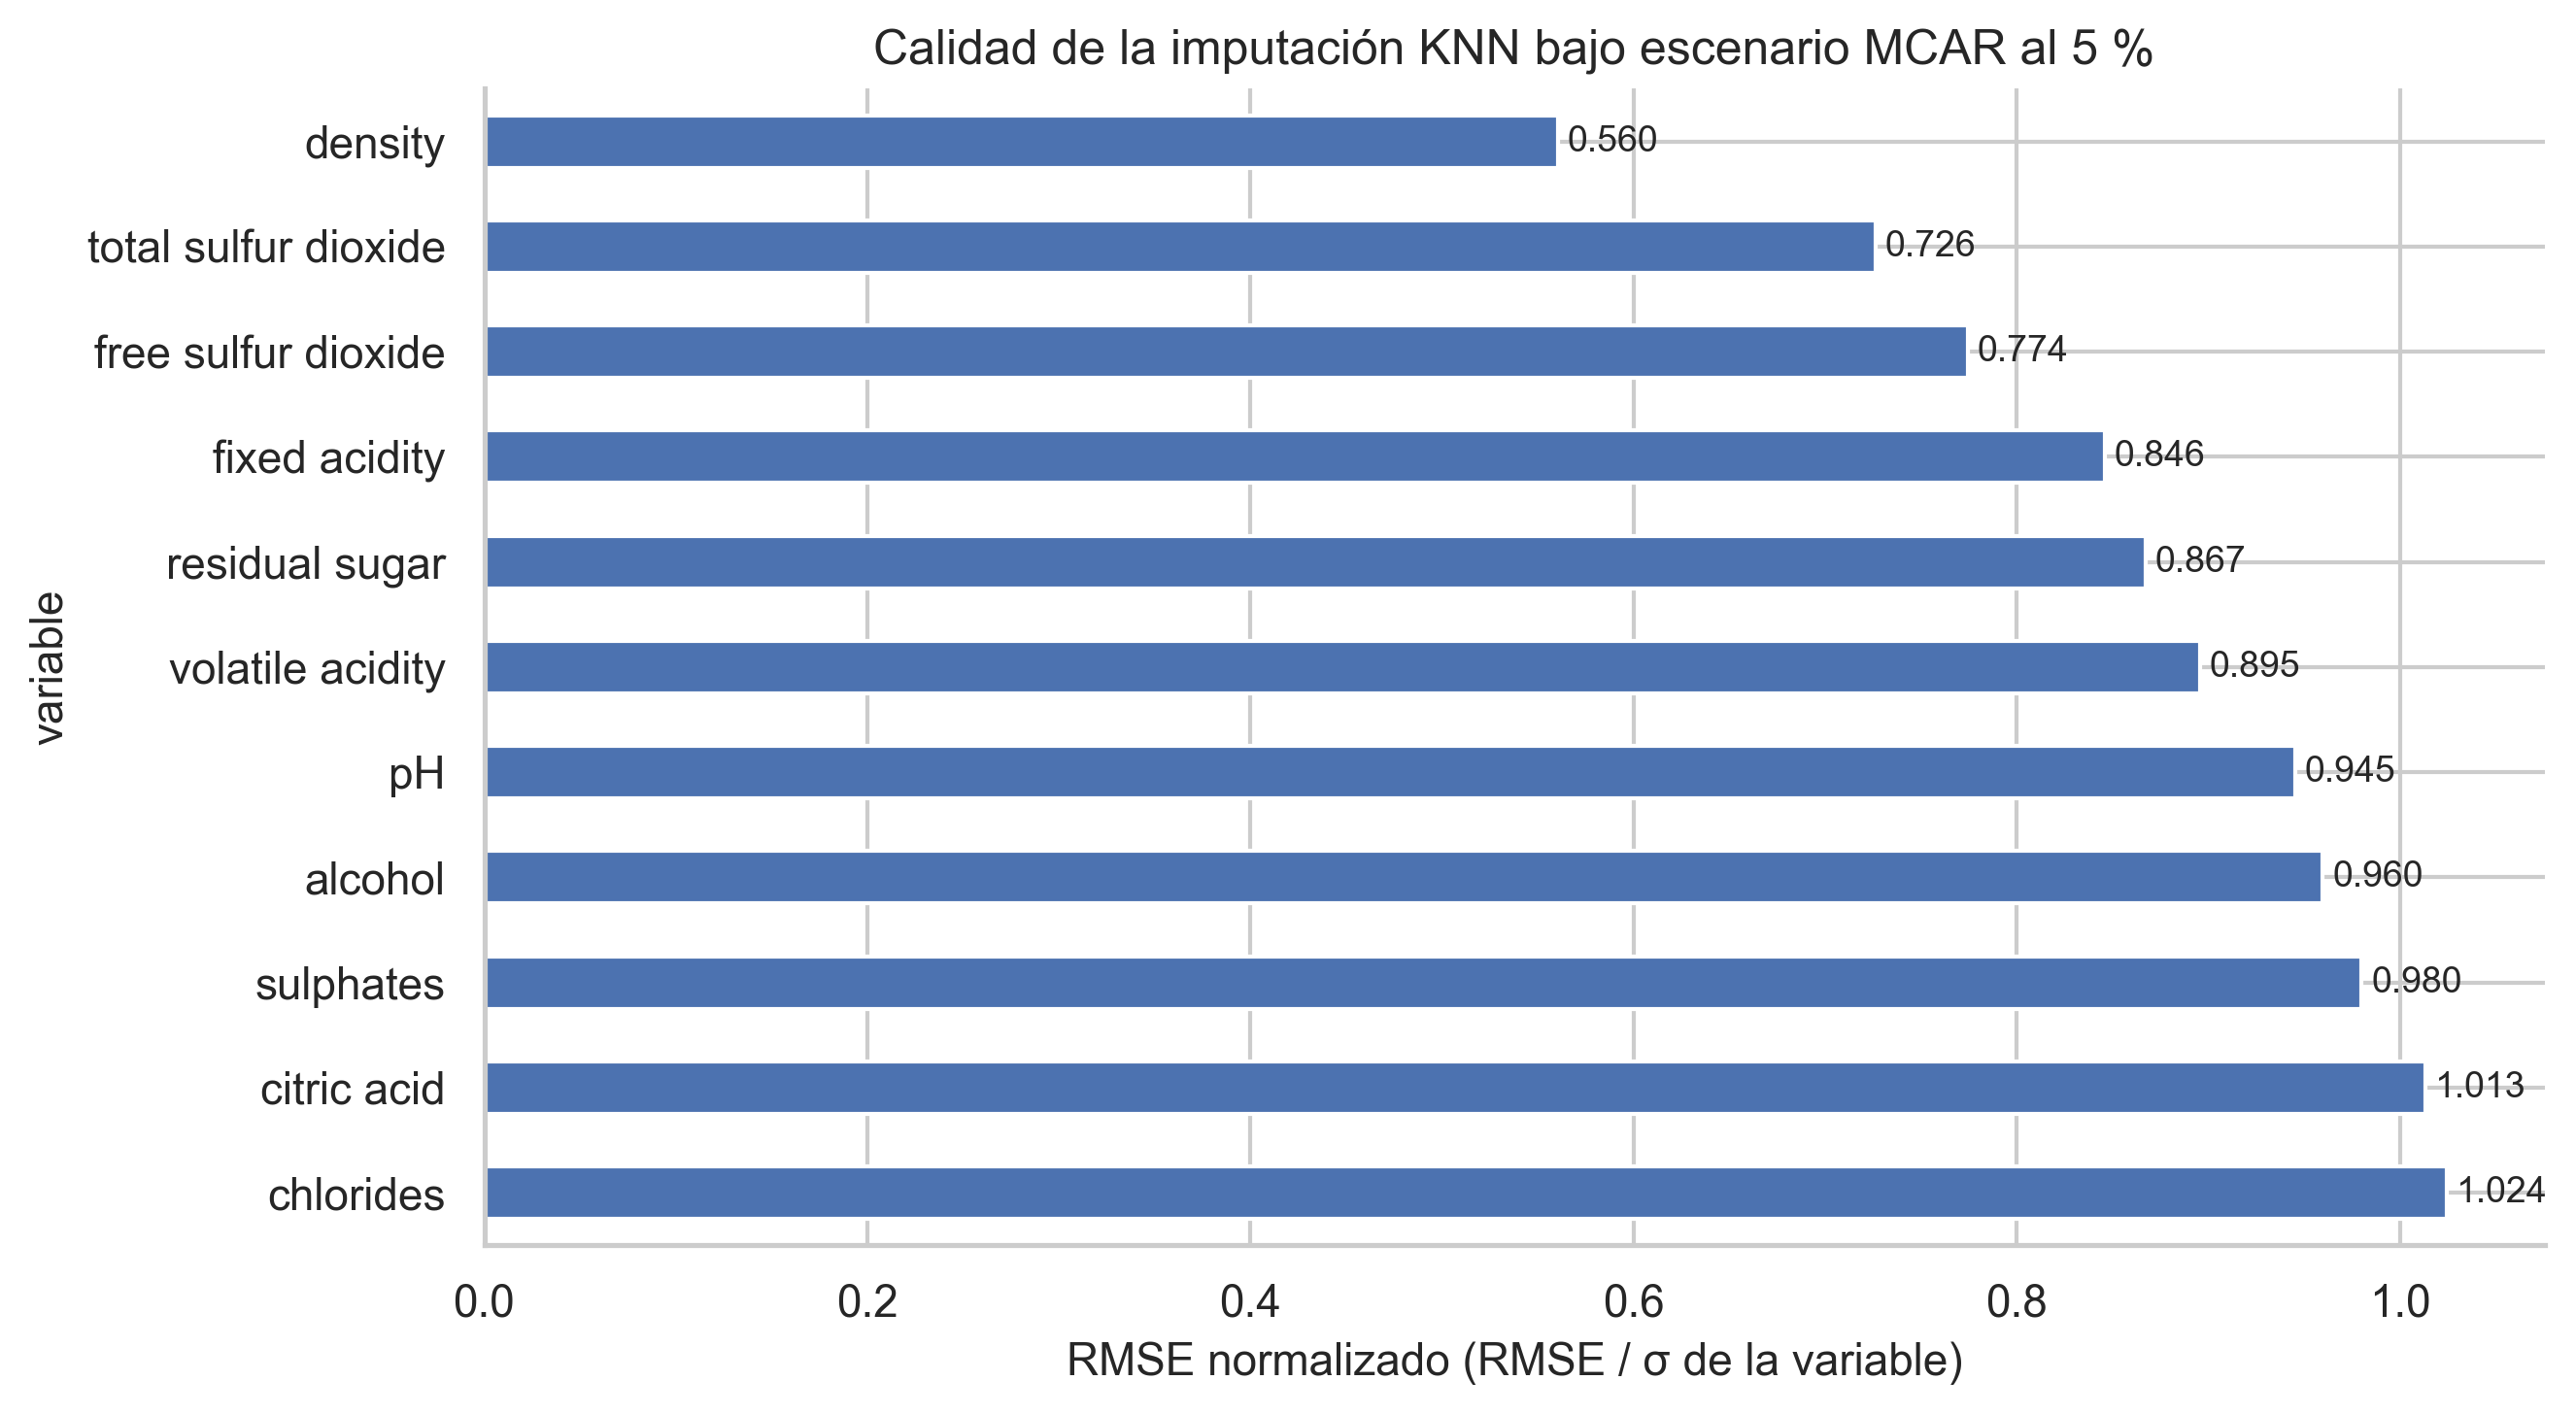
\includegraphics[width=\columnwidth]{fig_u4_01_imputacion_knn.png}
    \caption{Validación de la imputación KNN sobre el escenario MCAR
             simulado al 5\,\%. Los valores imputados (naranja) reproducen
             la distribución original (azul) con error reducido.}
    \label{fig:imputacion-knn}
\end{figure}

La transformación Yeo--Johnson \cite{yeo2000power} se aplicó a
\texttt{chlorides}, \texttt{residual sugar} y \texttt{sulphates}, reduciendo
drásticamente su asimetría sin descartar observaciones, como se aprecia en
la Figura~\ref{fig:yeojohnson}. Tras la transformación, el
\texttt{StandardScaler} fue la opción más apropiada por producir
distribuciones centradas y con varianza unitaria, coherentes con análisis
posteriores basados en distancias o covarianzas
(Fig.~\ref{fig:escaladores}).

\begin{figure}[t]
    \centering
    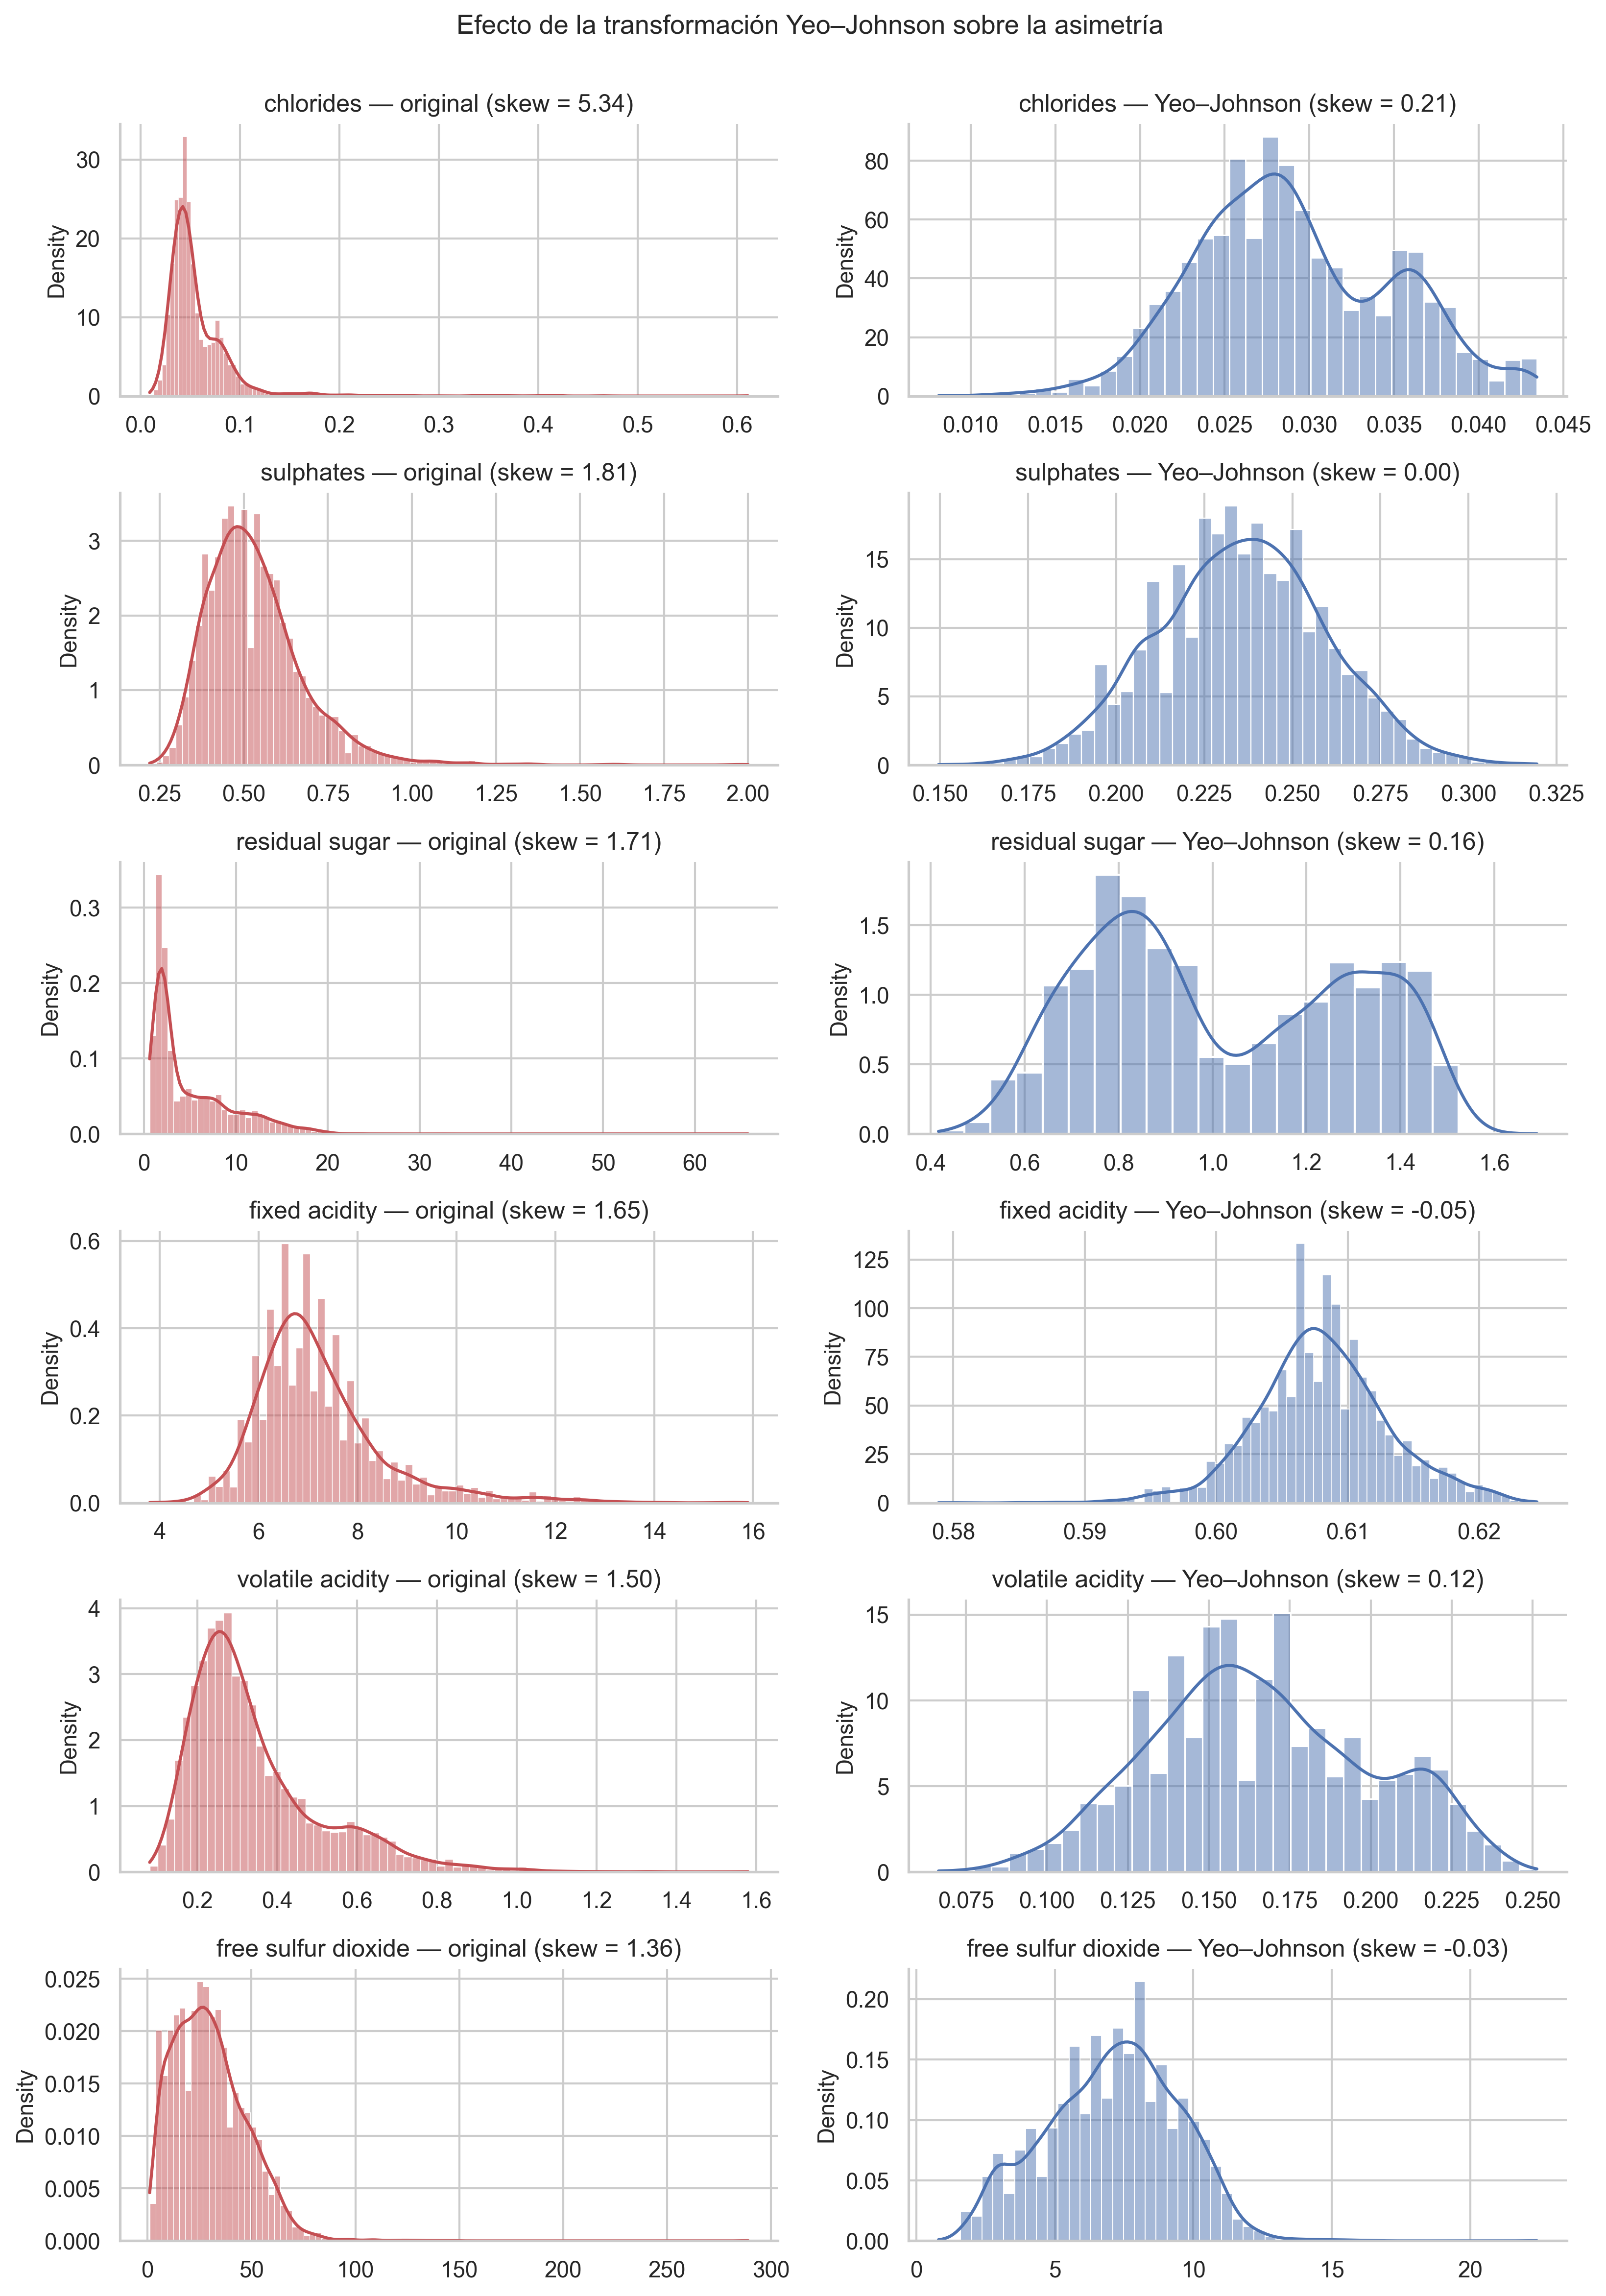
\includegraphics[width=\columnwidth]{fig_u4_02_yeojohnson.png}
    \caption{Efecto de la transformación Yeo--Johnson sobre las
             variables con mayor asimetría. Se observa una reducción
             considerable del sesgo y la elongación de las colas.}
    \label{fig:yeojohnson}
\end{figure}

\begin{figure}[t]
    \centering
    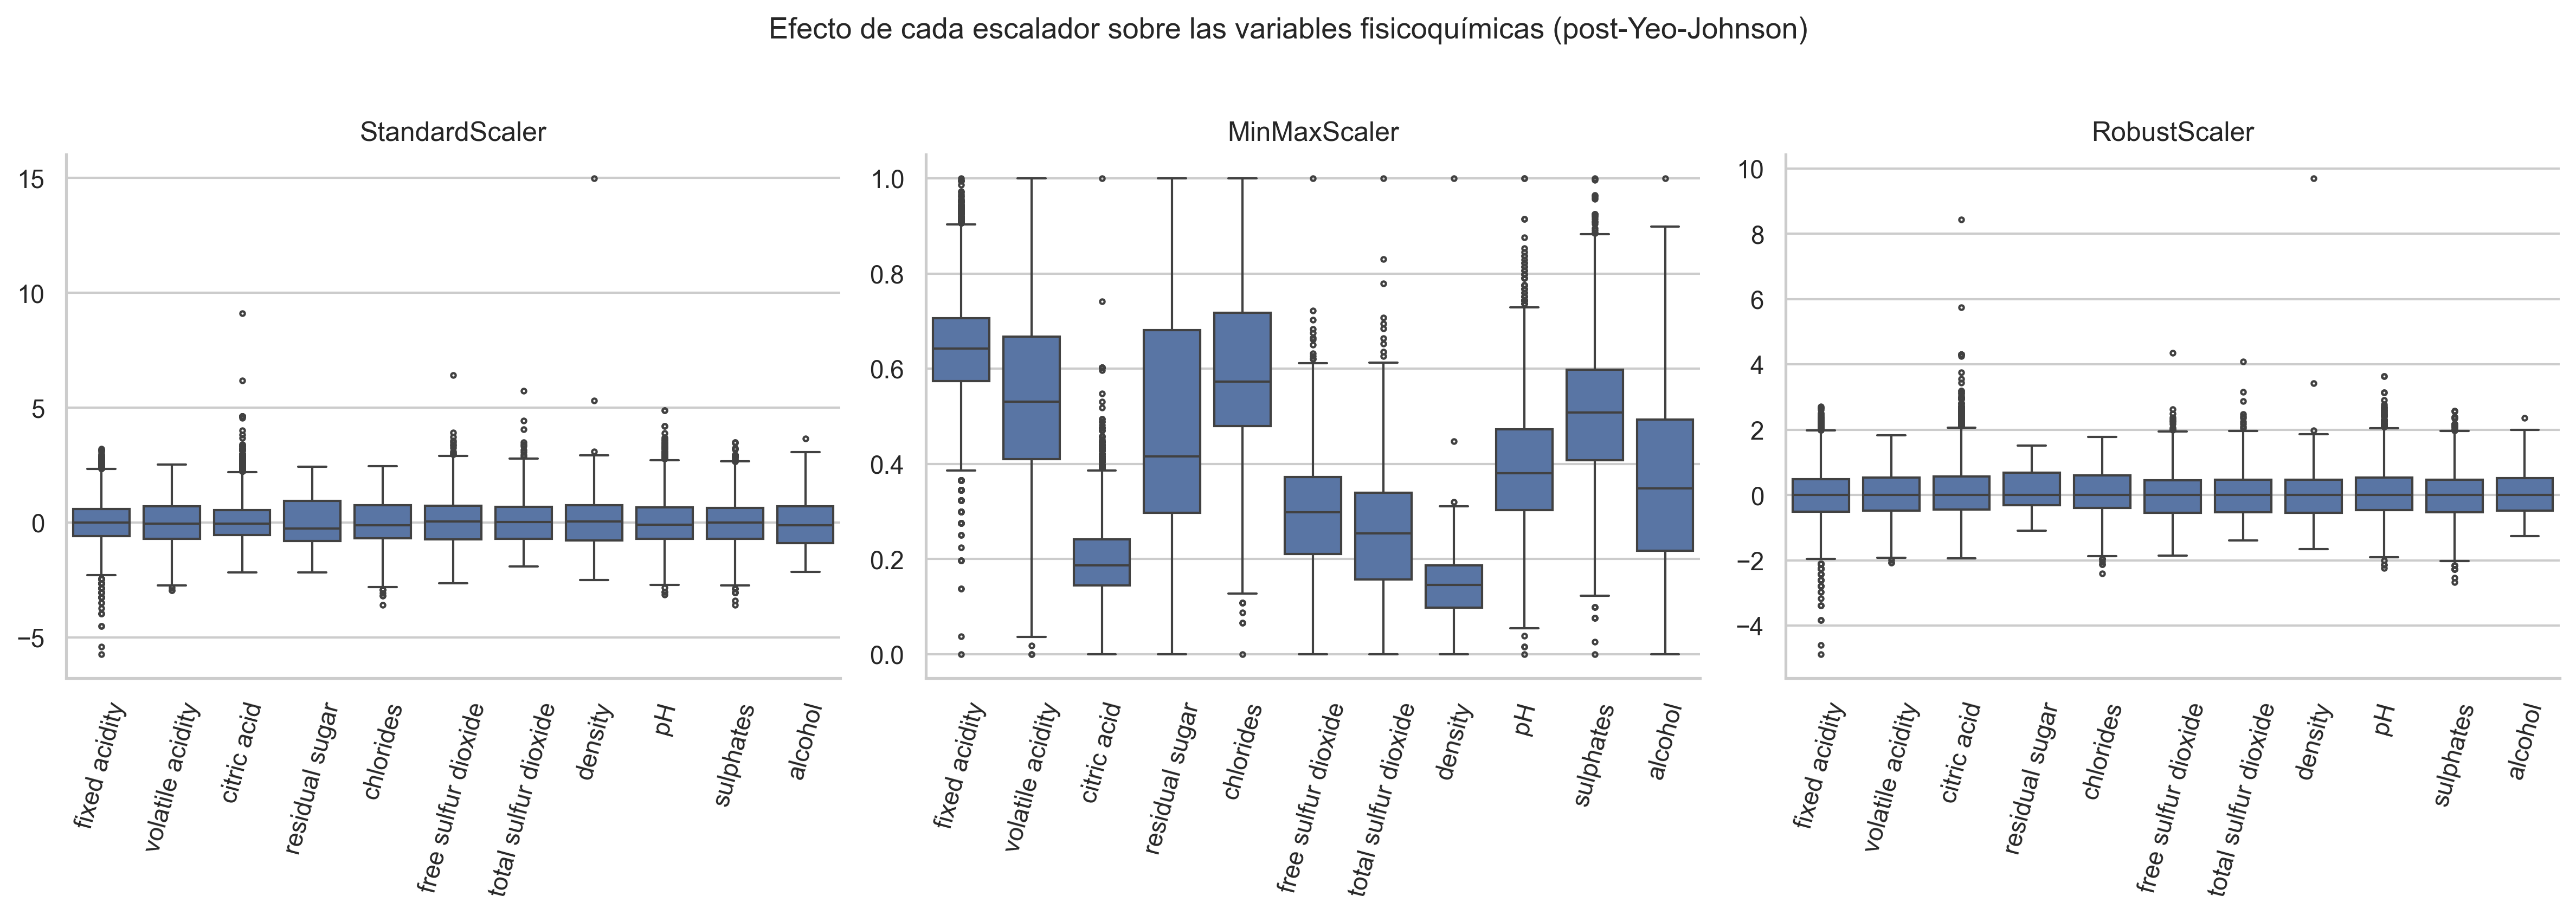
\includegraphics[width=\columnwidth]{fig_u4_03_escaladores.png}
    \caption{Comparación de StandardScaler, MinMaxScaler y RobustScaler
             aplicados al conjunto post-transformación.
             StandardScaler produce la distribución más equilibrada
             tras Yeo--Johnson.}
    \label{fig:escaladores}
\end{figure}

% ─────────────────────────────────────────────────────────────────────────────
\section{Conclusiones}
\label{sec:conclusiones}

Este trabajo realizó un análisis exploratorio completo del conjunto
\textit{Wine Quality}, cubriendo cuatro bloques metodológicos: análisis
exploratorio (univariado, bivariado y multivariado), detección de atípicos,
preprocesamiento y síntesis de hallazgos.

Los resultados principales son:

\begin{enumerate}
    \item \texttt{alcohol} es la variable con mayor asociación monótona con
    la calidad sensorial ($\rho_{\text{Spearman}} \approx 0{,}45$), seguida
    de \texttt{density} ($\rho \approx -0{,}32$) y \texttt{chlorides}
    ($\rho \approx -0{,}30$), patrón consistente con la literatura original
    del dataset \cite{cortez2009wine}.

    \item El PCA revela que la principal fuente de varianza (PC1, 27,5\,\%)
    es el contraste químico entre vinos tintos y blancos, no la calidad. El
    gradiente de calidad en el espacio reducido es difuso, lo que anticipa la
    necesidad de modelos no lineales para predecirla (árboles, ensambles).

    \item La asociación entre tipo de vino y calidad, aunque estadísticamente
    significativa, es débil (V de Cramér $\approx 0{,}09$): el tipo influye
    pero no determina la calidad percibida.

    \item Los métodos univariados (IQR, $Z$-score) y multivariados (Isolation
    Forest \cite{liu2008iforest}, LOF \cite{breunig2000lof}) capturan
    geometrías distintas de anomalía. La decisión de conservar los atípicos
    univariados, compensando su efecto con Yeo--Johnson, es metodológicamente
    sólida dado el carácter legítimo de los valores extremos en datos
    vitivinícolas.

    \item El flujo \textit{deduplicar $\rightarrow$ imputar $\rightarrow$
    transformar $\rightarrow$ escalar} produce un conjunto de 5\,320
    observaciones consistente, centrado y con varianza unitaria, listo para
    modelado supervisado.
\end{enumerate}

\textbf{Limitaciones.} El análisis es exclusivamente exploratorio: no se
construyó ni validó ningún modelo predictivo. Los vinos provienen de una única
región (\textit{Vinho Verde}, Portugal) y de una única ventana temporal, por
lo que los hallazgos pueden no generalizar a otros estilos. El fuerte desbalance
ordinal de \texttt{quality} (90\,\% en clases 5--7) condicionará cualquier
modelado posterior.

\textbf{Trabajo futuro.} Las líneas naturales de continuación incluyen: (i)
modelado supervisado de \texttt{quality} con árboles de decisión, ensambles y
validación cruzada estratificada; (ii)~tratamiento explícito del desbalance
ordinal (SMOTE, ponderación de clases); (iii)~análisis estratificado por tipo
de vino; e (iv)~ingeniería de variables con ratios fisicoquímicos relevantes.

% ─────────────────────────────────────────────────────────────────────────────
\section*{Consideraciones éticas y disponibilidad de datos}

El conjunto \textit{Wine Quality} fue publicado bajo licencia abierta por
Cortez et al.\ \cite{cortez2009wine} en el UCI Machine Learning Repository
\cite{uci_repo}. Los datos corresponden exclusivamente a mediciones químicas
y calificaciones sensoriales agregadas; no contienen información personal ni
de identificación. El código fuente, el notebook y el conjunto procesado están
disponibles en el repositorio público del proyecto:
\url{https://github.com/caamilo03/wine-quality}.

% ─────────────────────────────────────────────────────────────────────────────
\bibliographystyle{IEEEtran}
\bibliography{refs}

\end{document}
